% Options for packages loaded elsewhere
\PassOptionsToPackage{unicode}{hyperref}
\PassOptionsToPackage{hyphens}{url}
\PassOptionsToPackage{dvipsnames,svgnames,x11names}{xcolor}
%
\documentclass[
  letterpaper,
  DIV=11,
  numbers=noendperiod]{scrartcl}

\usepackage{amsmath,amssymb}
\usepackage{iftex}
\ifPDFTeX
  \usepackage[T1]{fontenc}
  \usepackage[utf8]{inputenc}
  \usepackage{textcomp} % provide euro and other symbols
\else % if luatex or xetex
  \usepackage{unicode-math}
  \defaultfontfeatures{Scale=MatchLowercase}
  \defaultfontfeatures[\rmfamily]{Ligatures=TeX,Scale=1}
\fi
\usepackage{lmodern}
\ifPDFTeX\else  
    % xetex/luatex font selection
\fi
% Use upquote if available, for straight quotes in verbatim environments
\IfFileExists{upquote.sty}{\usepackage{upquote}}{}
\IfFileExists{microtype.sty}{% use microtype if available
  \usepackage[]{microtype}
  \UseMicrotypeSet[protrusion]{basicmath} % disable protrusion for tt fonts
}{}
\makeatletter
\@ifundefined{KOMAClassName}{% if non-KOMA class
  \IfFileExists{parskip.sty}{%
    \usepackage{parskip}
  }{% else
    \setlength{\parindent}{0pt}
    \setlength{\parskip}{6pt plus 2pt minus 1pt}}
}{% if KOMA class
  \KOMAoptions{parskip=half}}
\makeatother
\usepackage{xcolor}
\usepackage[top=1.54cm, bottom=1.94cm, left=1.54cm,
right=1.54cm]{geometry}
\setlength{\emergencystretch}{3em} % prevent overfull lines
\setcounter{secnumdepth}{-\maxdimen} % remove section numbering
% Make \paragraph and \subparagraph free-standing
\makeatletter
\ifx\paragraph\undefined\else
  \let\oldparagraph\paragraph
  \renewcommand{\paragraph}{
    \@ifstar
      \xxxParagraphStar
      \xxxParagraphNoStar
  }
  \newcommand{\xxxParagraphStar}[1]{\oldparagraph*{#1}\mbox{}}
  \newcommand{\xxxParagraphNoStar}[1]{\oldparagraph{#1}\mbox{}}
\fi
\ifx\subparagraph\undefined\else
  \let\oldsubparagraph\subparagraph
  \renewcommand{\subparagraph}{
    \@ifstar
      \xxxSubParagraphStar
      \xxxSubParagraphNoStar
  }
  \newcommand{\xxxSubParagraphStar}[1]{\oldsubparagraph*{#1}\mbox{}}
  \newcommand{\xxxSubParagraphNoStar}[1]{\oldsubparagraph{#1}\mbox{}}
\fi
\makeatother

\usepackage{color}
\usepackage{fancyvrb}
\newcommand{\VerbBar}{|}
\newcommand{\VERB}{\Verb[commandchars=\\\{\}]}
\DefineVerbatimEnvironment{Highlighting}{Verbatim}{commandchars=\\\{\}}
% Add ',fontsize=\small' for more characters per line
\usepackage{framed}
\definecolor{shadecolor}{RGB}{241,243,245}
\newenvironment{Shaded}{\begin{snugshade}}{\end{snugshade}}
\newcommand{\AlertTok}[1]{\textcolor[rgb]{0.68,0.00,0.00}{#1}}
\newcommand{\AnnotationTok}[1]{\textcolor[rgb]{0.37,0.37,0.37}{#1}}
\newcommand{\AttributeTok}[1]{\textcolor[rgb]{0.40,0.45,0.13}{#1}}
\newcommand{\BaseNTok}[1]{\textcolor[rgb]{0.68,0.00,0.00}{#1}}
\newcommand{\BuiltInTok}[1]{\textcolor[rgb]{0.00,0.23,0.31}{#1}}
\newcommand{\CharTok}[1]{\textcolor[rgb]{0.13,0.47,0.30}{#1}}
\newcommand{\CommentTok}[1]{\textcolor[rgb]{0.37,0.37,0.37}{#1}}
\newcommand{\CommentVarTok}[1]{\textcolor[rgb]{0.37,0.37,0.37}{\textit{#1}}}
\newcommand{\ConstantTok}[1]{\textcolor[rgb]{0.56,0.35,0.01}{#1}}
\newcommand{\ControlFlowTok}[1]{\textcolor[rgb]{0.00,0.23,0.31}{\textbf{#1}}}
\newcommand{\DataTypeTok}[1]{\textcolor[rgb]{0.68,0.00,0.00}{#1}}
\newcommand{\DecValTok}[1]{\textcolor[rgb]{0.68,0.00,0.00}{#1}}
\newcommand{\DocumentationTok}[1]{\textcolor[rgb]{0.37,0.37,0.37}{\textit{#1}}}
\newcommand{\ErrorTok}[1]{\textcolor[rgb]{0.68,0.00,0.00}{#1}}
\newcommand{\ExtensionTok}[1]{\textcolor[rgb]{0.00,0.23,0.31}{#1}}
\newcommand{\FloatTok}[1]{\textcolor[rgb]{0.68,0.00,0.00}{#1}}
\newcommand{\FunctionTok}[1]{\textcolor[rgb]{0.28,0.35,0.67}{#1}}
\newcommand{\ImportTok}[1]{\textcolor[rgb]{0.00,0.46,0.62}{#1}}
\newcommand{\InformationTok}[1]{\textcolor[rgb]{0.37,0.37,0.37}{#1}}
\newcommand{\KeywordTok}[1]{\textcolor[rgb]{0.00,0.23,0.31}{\textbf{#1}}}
\newcommand{\NormalTok}[1]{\textcolor[rgb]{0.00,0.23,0.31}{#1}}
\newcommand{\OperatorTok}[1]{\textcolor[rgb]{0.37,0.37,0.37}{#1}}
\newcommand{\OtherTok}[1]{\textcolor[rgb]{0.00,0.23,0.31}{#1}}
\newcommand{\PreprocessorTok}[1]{\textcolor[rgb]{0.68,0.00,0.00}{#1}}
\newcommand{\RegionMarkerTok}[1]{\textcolor[rgb]{0.00,0.23,0.31}{#1}}
\newcommand{\SpecialCharTok}[1]{\textcolor[rgb]{0.37,0.37,0.37}{#1}}
\newcommand{\SpecialStringTok}[1]{\textcolor[rgb]{0.13,0.47,0.30}{#1}}
\newcommand{\StringTok}[1]{\textcolor[rgb]{0.13,0.47,0.30}{#1}}
\newcommand{\VariableTok}[1]{\textcolor[rgb]{0.07,0.07,0.07}{#1}}
\newcommand{\VerbatimStringTok}[1]{\textcolor[rgb]{0.13,0.47,0.30}{#1}}
\newcommand{\WarningTok}[1]{\textcolor[rgb]{0.37,0.37,0.37}{\textit{#1}}}

\providecommand{\tightlist}{%
  \setlength{\itemsep}{0pt}\setlength{\parskip}{0pt}}\usepackage{longtable,booktabs,array}
\usepackage{calc} % for calculating minipage widths
% Correct order of tables after \paragraph or \subparagraph
\usepackage{etoolbox}
\makeatletter
\patchcmd\longtable{\par}{\if@noskipsec\mbox{}\fi\par}{}{}
\makeatother
% Allow footnotes in longtable head/foot
\IfFileExists{footnotehyper.sty}{\usepackage{footnotehyper}}{\usepackage{footnote}}
\makesavenoteenv{longtable}
\usepackage{graphicx}
\makeatletter
\newsavebox\pandoc@box
\newcommand*\pandocbounded[1]{% scales image to fit in text height/width
  \sbox\pandoc@box{#1}%
  \Gscale@div\@tempa{\textheight}{\dimexpr\ht\pandoc@box+\dp\pandoc@box\relax}%
  \Gscale@div\@tempb{\linewidth}{\wd\pandoc@box}%
  \ifdim\@tempb\p@<\@tempa\p@\let\@tempa\@tempb\fi% select the smaller of both
  \ifdim\@tempa\p@<\p@\scalebox{\@tempa}{\usebox\pandoc@box}%
  \else\usebox{\pandoc@box}%
  \fi%
}
% Set default figure placement to htbp
\def\fps@figure{htbp}
\makeatother
% definitions for citeproc citations
\NewDocumentCommand\citeproctext{}{}
\NewDocumentCommand\citeproc{mm}{%
  \begingroup\def\citeproctext{#2}\cite{#1}\endgroup}
\makeatletter
 % allow citations to break across lines
 \let\@cite@ofmt\@firstofone
 % avoid brackets around text for \cite:
 \def\@biblabel#1{}
 \def\@cite#1#2{{#1\if@tempswa , #2\fi}}
\makeatother
\newlength{\cslhangindent}
\setlength{\cslhangindent}{1.5em}
\newlength{\csllabelwidth}
\setlength{\csllabelwidth}{3em}
\newenvironment{CSLReferences}[2] % #1 hanging-indent, #2 entry-spacing
 {\begin{list}{}{%
  \setlength{\itemindent}{0pt}
  \setlength{\leftmargin}{0pt}
  \setlength{\parsep}{0pt}
  % turn on hanging indent if param 1 is 1
  \ifodd #1
   \setlength{\leftmargin}{\cslhangindent}
   \setlength{\itemindent}{-1\cslhangindent}
  \fi
  % set entry spacing
  \setlength{\itemsep}{#2\baselineskip}}}
 {\end{list}}
\usepackage{calc}
\newcommand{\CSLBlock}[1]{\hfill\break\parbox[t]{\linewidth}{\strut\ignorespaces#1\strut}}
\newcommand{\CSLLeftMargin}[1]{\parbox[t]{\csllabelwidth}{\strut#1\strut}}
\newcommand{\CSLRightInline}[1]{\parbox[t]{\linewidth - \csllabelwidth}{\strut#1\strut}}
\newcommand{\CSLIndent}[1]{\hspace{\cslhangindent}#1}

\usepackage{booktabs}
\usepackage{longtable}
\usepackage{array}
\usepackage{multirow}
\usepackage{wrapfig}
\usepackage{float}
\usepackage{colortbl}
\usepackage{pdflscape}
\usepackage{tabu}
\usepackage{threeparttable}
\usepackage{threeparttablex}
\usepackage[normalem]{ulem}
\usepackage{makecell}
\usepackage{xcolor}
\usepackage{amsmath}
\usepackage{fvextra}
\usepackage{pdflscape}
\DefineVerbatimEnvironment{Highlighting}{Verbatim}{breaklines,commandchars=\\\{\}}
\DefineVerbatimEnvironment{OutputCode}{Verbatim}{breaklines,commandchars=\\\{\}}
\KOMAoption{captions}{tableheading}
\makeatletter
\@ifpackageloaded{caption}{}{\usepackage{caption}}
\AtBeginDocument{%
\ifdefined\contentsname
  \renewcommand*\contentsname{Table of contents}
\else
  \newcommand\contentsname{Table of contents}
\fi
\ifdefined\listfigurename
  \renewcommand*\listfigurename{List of Figures}
\else
  \newcommand\listfigurename{List of Figures}
\fi
\ifdefined\listtablename
  \renewcommand*\listtablename{List of Tables}
\else
  \newcommand\listtablename{List of Tables}
\fi
\ifdefined\figurename
  \renewcommand*\figurename{Figure}
\else
  \newcommand\figurename{Figure}
\fi
\ifdefined\tablename
  \renewcommand*\tablename{Table}
\else
  \newcommand\tablename{Table}
\fi
}
\@ifpackageloaded{float}{}{\usepackage{float}}
\floatstyle{ruled}
\@ifundefined{c@chapter}{\newfloat{codelisting}{h}{lop}}{\newfloat{codelisting}{h}{lop}[chapter]}
\floatname{codelisting}{Listing}
\newcommand*\listoflistings{\listof{codelisting}{List of Listings}}
\makeatother
\makeatletter
\makeatother
\makeatletter
\@ifpackageloaded{caption}{}{\usepackage{caption}}
\@ifpackageloaded{subcaption}{}{\usepackage{subcaption}}
\makeatother

\usepackage{bookmark}

\IfFileExists{xurl.sty}{\usepackage{xurl}}{} % add URL line breaks if available
\urlstyle{same} % disable monospaced font for URLs
\hypersetup{
  pdftitle={Evaluating Missing Data Handling Techniques Under Different Missingness Mechanisms},
  pdfauthor={Rophence Ojiambo; Kiran Nagdeo; Cindy Patippe},
  colorlinks=true,
  linkcolor={blue},
  filecolor={Maroon},
  citecolor={Blue},
  urlcolor={blue},
  pdfcreator={LaTeX via pandoc}}


\title{Evaluating Missing Data Handling Techniques Under Different
Missingness Mechanisms}
\author{Rophence Ojiambo \and Kiran Nagdeo \and Cindy Patippe}
\date{}

\begin{document}
\maketitle


\section{Introduction}\label{introduction}

\subsubsection{Overview of Missingness
Mechanisms}\label{overview-of-missingness-mechanisms}

Missing data, whether due to corruption or logistical issues, can bias
estimates, inflate standard errors, and invalidate inferences if not
properly
handled\textsuperscript{{[}\citeproc{ref-rubin1987statistical}{1}{]}}.
Rubin's (1976)
framework\textsuperscript{{[}\citeproc{ref-rubin1976inference}{2}{]}}
defines three mechanisms: Missing Completely at Random (MCAR), where
missingness is unrelated to any data; Missing at Random (MAR), where
missingness depends only on observed data; and Missing Not at Random
(MNAR), where missingness depends on unobserved values, posing the
greatest challenge and requiring strong, often unverifiable
assumptions\textsuperscript{{[}\citeproc{ref-enders2022applied}{3}{]}}.
Complete-case analysis is commonly used in applied research for its
simplicity, but under MAR or MNAR conditions, it can introduce bias and
reduce
efficiency\textsuperscript{{[}\citeproc{ref-schafer2002missing}{4}{]}}.
Single imputation methods (e.g., mean substitution) also perform poorly,
distorting distributions and underestimating uncertainty. In contrast,
Multiple Imputation by Chained Equations (MICE) and related model-based
approaches simulate missing values multiple times and pool results to
reflect imputation
uncertainty\textsuperscript{{[}\citeproc{ref-van2011mice}{5}{]}}. While
increasingly popular, the performance of these methods varies depending
on the nature and extent of missingness
mechanism\textsuperscript{{[}\citeproc{ref-donders2006gentle}{6}{]}}.
Simulation studies allow systematic evaluation of these methods by
generating complete data, imposing missingness mechanisms, and comparing
outcomes such as bias, confidence interval coverage, prediction
accuracy, and model fit (e.g., AIC,
BIC)\textsuperscript{{[}\citeproc{ref-audigier2016principal}{7},\citeproc{ref-carpenter2023multiple}{8}{]}}.

\subsubsection{Relevance to Obesity
Research}\label{relevance-to-obesity-research}

Obesity presents a growing public health challenge worldwide,
contributing to increased risk of cardiovascular disease, type 2
diabetes, hypertension, musculoskeletal disorders, and certain cancers.
According to the World Health Organization
(2024)\textsuperscript{{[}\citeproc{ref-world2024obesity}{9}{]}}, global
obesity prevalence has tripled since 1975, and over 650 million adults
are currently classified as obese. In Latin America, where countries
like Mexico, Peru, and Colombia are experiencing rapid nutrition and
lifestyle transitions, obesity rates have surged across all age
groups\textsuperscript{{[}\citeproc{ref-rivera2014childhood}{10}--\citeproc{ref-food2019drink}{12}{]}}.
The determinants of obesity are multifactorial, including
sociodemographic variables, poor dietary patterns, inadequate physical
activity, sedentary behaviors, and harmful habits such as smoking and
alcohol
consumption\textsuperscript{{[}\citeproc{ref-palechor2019dataset}{13},\citeproc{ref-de2019obesity}{14}{]}}.
These risk factors are often collected via self-report or web-based
tools, making them especially vulnerable to missingness due to social
desirability bias, recall error, or issues with technology access.
Understanding how missing data may bias the estimation of such
relationships is critical for valid epidemiologic inference.

\subsubsection{Study Objective}\label{study-objective}

The objective of this project is to conduct a simulation study using the
\href{https://archive.ics.uci.edu/dataset/544/estimation+of+obesity+levels+based+on+eating+habits+and+physical+condition}{UCI
Obesity} dataset to assess how various imputation techniques perform
under MCAR, MAR, and MNAR scenarios.

\newpage

\section{Methods}\label{methods}

\subsection{Data Source}\label{data-source}

We used the \texttt{obesity.levels} dataset from the \texttt{fairml} R
package, which contains 2,111 records from individuals in Mexico, Peru,
and Colombia. The dataset includes 17 demographic, behavioral, and
physical condition attributes used to estimate obesity levels, labeled
by the \texttt{NObeyesdad} variable. Approximately 77\% of the data were
synthetically generated using Weka and SMOTE, while 23\% were collected
via a web platform. Further details are
elsewhere\textsuperscript{{[}\citeproc{ref-palechor2019dataset}{13},\citeproc{ref-de2019obesity}{14}{]}}.
The binary outcome variable, denoted as \texttt{Obesity}, was derived
from the original multiclass label \texttt{NObeyesdad} by coding
individuals with Obesity Type I, II, or III as ``Obese'' and others as
``Not Obese''. Continuous predictors included: Age, \texttt{FCVC}
(Frequency of vegetable consumption), \texttt{NCP} (Number of main
meals), \texttt{CH2O} (daily water intake), \texttt{FAF} (physical
activity frequency), and \texttt{TUE} (time using technology).
Categorical variables included Gender, family history with overweight,
high-calorie food consumption (\texttt{FAVC}), food between meals
(\texttt{CAEC}), smoking (\texttt{SMOKE}), calorie monitoring
(\texttt{SCC}), alcohol consumption (\texttt{CALC}), and transportation
type (\texttt{MTRANS}).

\subsection{Missing Data Generation
Mechanisms}\label{missing-data-generation-mechanisms}

We simulated missingness under three mechanisms: To simulate MCAR, we
randomly introduced missing values in three variables; \texttt{Gender},
\texttt{FAF}, and \texttt{CH2O}, with predefined rates of 15\%, 25\%,
and 20\%, respectively. The probability of missingness in these
variables is independent of any observed or unobserved data. We
simulated MAR by conditioning missingness on observed covariates.
Specifically: \texttt{FAF} was more likely to be missing for older
males; \texttt{SCC} was more likely to be missing among participants
reporting high-calorie food consumption; \texttt{NCP} was more likely to
be missing for younger females. Probabilities of missingness were
generated using logistic functions of these predictors.For MNAR,
missingness depended on unobserved (true) values of the variables
themselves: \texttt{FAF} missingness was more likely in individuals with
low physical activity; \texttt{CALC} was more likely missing in frequent
drinkers; \texttt{SCC} missingness was higher among participants who did
not monitor calories. These dependencies reflect real-world challenges
where values themselves influence their probability of being missing.

\subsection{Imputation Methods}\label{imputation-methods}

We applied three common strategies to handle missing data; (1) Complete
Case Analysis where all records with missing values in any of the
selected predictors were excluded; (2) Mean/Mode Imputation where for
continuous variables, missing values were imputed using the mean of
observed values and for categorical variables, the most frequent
category (mode) was used; (3) MICE using the \texttt{mice} package was
used to perform 5 multiple imputations using chained equations.

\subsection{Model Fitting and
Evaluation}\label{model-fitting-and-evaluation}

We trained logistic regression models to predict \texttt{Obesity} across
all datasets (Original, MCAR, MAR, MNAR) and imputation methods. Each
dataset was split into training (70\%) and test (30\%) sets using
stratified sampling to preserve the outcome distribution. Model
performance was evaluated using the following metrics:
\textbf{Accuracy:} Proportion of correct classifications;
\textbf{Sensitivity (Recall):} Proportion of obese individuals correctly
identified; \textbf{Specificity:} Proportion of non-obese individuals
correctly identified; \textbf{Area Under the ROC Curve (AUC):}
Discriminative ability of the model; \textbf{F1 Score:} Harmonic mean of
precision and recall. Model metrics were computed separately for the
training and test sets. For MICE, pooled predictions across imputations
were used for test metrics, and average metrics were reported for
training.

\newpage

\section{Results}\label{results}

\subsubsection{Exploratory Data
Analysis}\label{exploratory-data-analysis}

We conducted exploratory analysis to examine predictor distributions and
associations by obesity status. The outcome was moderately balanced
(54\% Not Obese, 46\% Obese). A correlation plot revealed notable
differences by class; for example, \texttt{Age} and \texttt{TUE} were
negatively correlated (r = --0.297 overall), more so among obese
participants. Relationships between \texttt{FCVC} and \texttt{NCP} also
varied across groups.

\begin{figure}[H]

{\centering 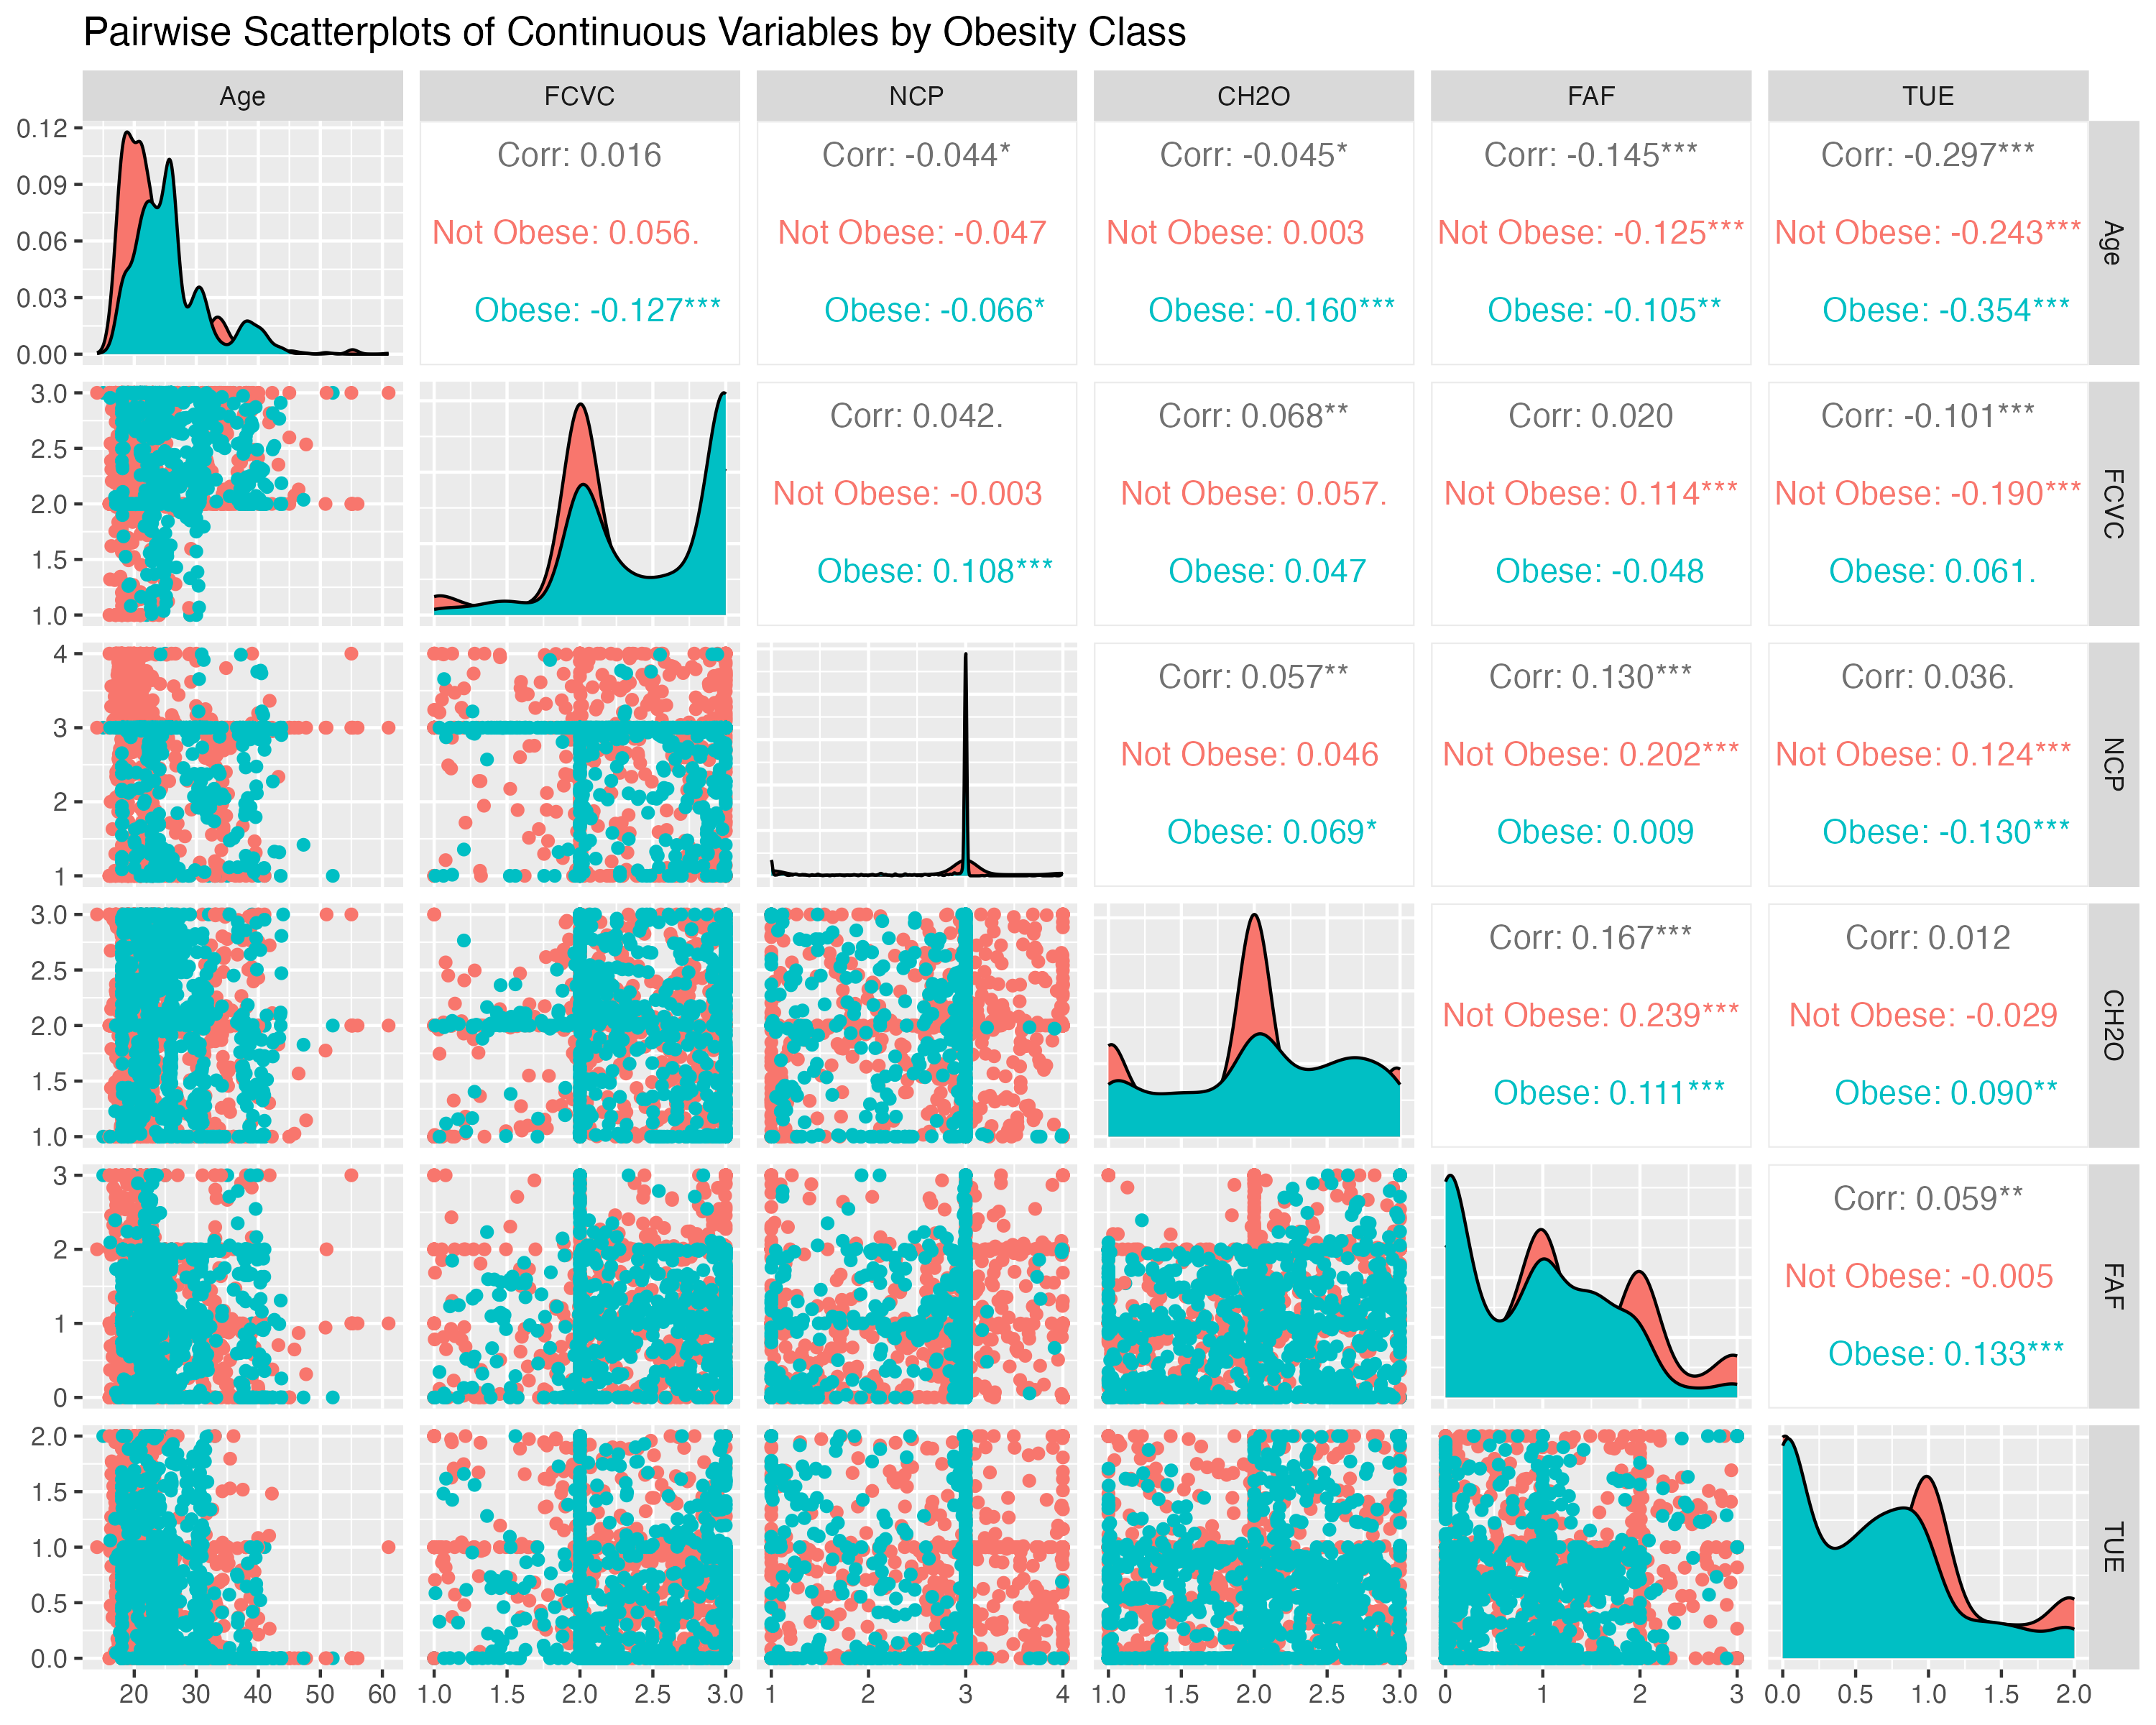
\includegraphics[width=1\linewidth,height=\textheight,keepaspectratio]{Analysis/pairs_plot.png}

}

\caption{Exploratory Data Analysis of Continuous Predictors by Obesity
Status}

\end{figure}%

We used Little's MCAR test (\texttt{naniar}, \texttt{misty}) to assess
missingness in the simulated dataset. Results (\(\chi^2 = 103.68\), df =
93, \(p = 0.211\)) suggest the data was consistent with MCAR. There were
8 unique missing patterns, with 1031 of 2111 cases missing at least one
value. Formal tests for MAR or MNAR were not possible; distinguishing
these mechanisms requires unverifiable assumptions or external data.
Missingness patterns are shown in the figure 2 below.

\begin{figure}[H]

{\centering 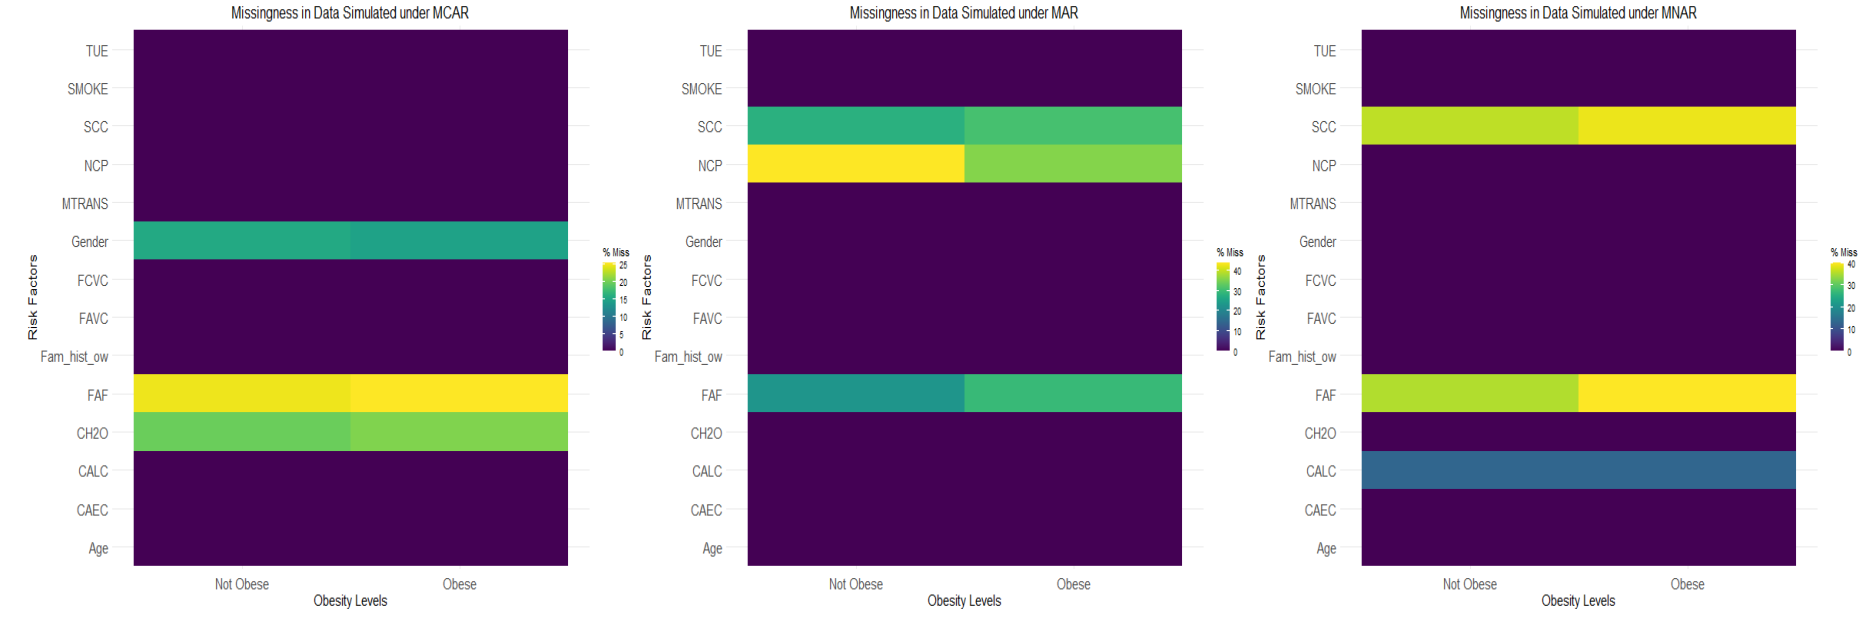
\includegraphics[width=1\linewidth,height=\textheight,keepaspectratio]{Analysis/missing_patterns.png}

}

\caption{Missingness Patterns under MCAR, MAR, and MNAR}

\end{figure}%

\subsubsection{Training Set Performance}\label{training-set-performance}

On the original full dataset without missing values, the model achieved
an accuracy of 77.5\%, sensitivity of 86.6\%, specificity of 69.7\%, and
an AUC of 0.8683. Under MCAR conditions, model performance varied only
slightly across imputation methods. Multiple imputation produced results
comparable to the original dataset (accuracy = 77.5\%, AUC = 0.8705),
whereas complete case analysis and mean/mode imputation led to modest
reductions in performance metrics. Notably, analysis with simulated data
under MCAR yielded an accuracy of 76.3\% and an AUC of 0.8642, see Table
1.

\begin{table}[H]
\centering
\caption{Model Performance on Training Set Across Missing Data Handling Methods}
\centering
\begin{tabular}[t]{llrrrrr}
\toprule
Scenario & Method & Accuracy & Sensitivity & Specificity & AUC & F1 Score\\
\midrule
\addlinespace[0.3em]
\multicolumn{7}{l}{\textbf{Full Dataset}}\\
\hspace{1em} & Original Dataset (No Missing) & 0.7748 & 0.8664 & 0.6967 & 0.8683 & 0.7799\\
\addlinespace[0.3em]
\multicolumn{7}{l}{\textbf{MCAR}}\\
\hspace{1em} & Simulated (with missing) & 0.7627 & 0.8612 & 0.6751 & 0.8642 & 0.7735\\
\hspace{1em} & Complete Case & 0.7649 & 0.8613 & 0.6837 & 0.8590 & 0.7700\\
\hspace{1em} & Mean/Mode Imputation & 0.7694 & 0.8576 & 0.6942 & 0.8691 & 0.7740\\
\hspace{1em} & Multiple Imputation (MICE) & 0.7753 & 0.8567 & 0.7058 & 0.8705 & 0.7783\\
\addlinespace[0.3em]
\multicolumn{7}{l}{\textbf{MAR}}\\
\hspace{1em} & Simulated (with missing) & 0.7813 & 0.8135 & 0.7561 & 0.8829 & 0.7659\\
\hspace{1em} & Complete Case & 0.8077 & 0.8182 & 0.7991 & 0.8871 & 0.7927\\
\hspace{1em} & Mean/Mode Imputation & 0.7769 & 0.8678 & 0.6992 & 0.8700 & 0.7817\\
\hspace{1em} & Multiple Imputation (MICE) & 0.7849 & 0.8658 & 0.7158 & 0.8700 & 0.7875\\
\addlinespace[0.3em]
\multicolumn{7}{l}{\textbf{MNAR}}\\
\hspace{1em} & Simulated (with missing) & 0.7550 & 0.8145 & 0.7082 & 0.8720 & 0.7453\\
\hspace{1em} & Complete Case & 0.7827 & 0.8505 & 0.7314 & 0.8865 & 0.7712\\
\hspace{1em} & Mean/Mode Imputation & 0.7647 & 0.8517 & 0.6905 & 0.8660 & 0.7692\\
\hspace{1em} & Multiple Imputation (MICE) & 0.7751 & 0.8614 & 0.7015 & 0.8678 & 0.7791\\
\bottomrule
\end{tabular}
\end{table}

In the MAR scenario, performance was more variable. Mean/mode imputation
and multiple imputation yielded high sensitivity (0.8678 and 0.8658,
respectively), but complete case analysis achieved the highest accuracy
(80.8\%) and AUC (0.8871). This may be due to selective retention of
more informative observations in the complete-case subset under the MAR
mechanism. Multiple imputation again demonstrated strong overall
performance with a balance of sensitivity and specificity. For the MNAR
scenario, overall performance was lower compared to MCAR and MAR, as
expected given the unidentifiability of the missing data mechanism
without further assumptions. Multiple imputation consistently
outperformed the other methods, closely matching the original dataset's
accuracy and AUC. Mean/Mode Imputation under MNAR led to the lowest AUC
(0.8660) among the imputation methods and lowest specificity (0.6905),
see Table 1 above.

\subsubsection{Test Set Performance}\label{test-set-performance}

Similar trends were observed in the test set evaluations. Under MCAR,
the highest sensitivity (90.7\%) was observed in the simulated dataset
with missingness. Multiple imputation again yielded performance close to
the original data (accuracy = 77.7\%, AUC = 0.8736), while complete case
analysis showed a slight increase in the AUC (0.8924)estimate, see Table
2 below. Under MAR, mean/mode imputation achieved the accuracy (77.7\%)
slightly above the original estimate and competitive AUC (0.8711),
albeit at the cost of lower specificity. Multiple imputation led to a
balanced trade-off across all metrics. In the MNAR setting, performance
was generally lower. The simulated incomplete data yielded an AUC of
0.8649, but this dropped to 0.8404 under complete-case analysis.
Nonetheless, MICE showed the most stable performance across all metrics
and missingness mechanisms, including MNAR, with an F1 Score of 0.7861
and accuracy of 78.6\%.

\begin{table}[H]
\centering
\caption{Model Performance on Test Set Across Missing Data Handling Methods}
\centering
\begin{tabular}[t]{llrrrrr}
\toprule
Scenario & Method & Accuracy & Sensitivity & Specificity & AUC & F1 Score\\
\midrule
\addlinespace[0.3em]
\multicolumn{7}{l}{\textbf{Full Dataset}}\\
\hspace{1em} & Original Dataset (No Missing) & 0.7753 & 0.8385 & 0.7214 & 0.8717 & 0.7746\\
\addlinespace[0.3em]
\multicolumn{7}{l}{\textbf{MCAR}}\\
\hspace{1em} & Simulated (with missing) & 0.7909 & 0.9071 & 0.7053 & 0.8862 & 0.7864\\
\hspace{1em} & Complete Case & 0.7740 & 0.8844 & 0.6818 & 0.8924 & 0.7808\\
\hspace{1em} & Mean/Mode Imputation & 0.7737 & 0.8488 & 0.7097 & 0.8717 & 0.7755\\
\hspace{1em} & Multiple Imputation (MICE) & 0.7769 & 0.8557 & 0.7097 & 0.8736 & 0.7793\\
\addlinespace[0.3em]
\multicolumn{7}{l}{\textbf{MAR}}\\
\hspace{1em} & Simulated (with missing) & 0.7987 & 0.8082 & 0.7901 & 0.8791 & 0.7919\\
\hspace{1em} & Complete Case & 0.7853 & 0.8354 & 0.7449 & 0.8776 & 0.7765\\
\hspace{1em} & Mean/Mode Imputation & 0.7769 & 0.8625 & 0.7038 & 0.8711 & 0.7807\\
\hspace{1em} & Multiple Imputation (MICE) & 0.7864 & 0.8660 & 0.7185 & 0.8770 & 0.7887\\
\addlinespace[0.3em]
\multicolumn{7}{l}{\textbf{MNAR}}\\
\hspace{1em} & Simulated (with missing) & 0.7476 & 0.8452 & 0.6803 & 0.8649 & 0.7320\\
\hspace{1em} & Complete Case & 0.7109 & 0.7692 & 0.6667 & 0.8404 & 0.6965\\
\hspace{1em} & Mean/Mode Imputation & 0.7816 & 0.8591 & 0.7155 & 0.8721 & 0.7837\\
\hspace{1em} & Multiple Imputation (MICE) & 0.7864 & 0.8522 & 0.7302 & 0.8765 & 0.7861\\
\bottomrule
\end{tabular}
\end{table}

\section{Conclusion}\label{conclusion}

Multiple imputation (MICE) showed the most consistent performance across
all missingness mechanisms. Complete case analysis performed well under
MAR but led to bias and data loss under MCAR and MNAR. Mean/mode
imputation was simple but less effective. These findings highlight the
need for principled approaches when missingness may not be MCAR.

\newpage

\section{Data Availabiliy}\label{data-availabiliy}

All codes and datasets for this project can be found at our
\href{https://github.com/rophenceojiambo/Simulations-Final-Project}{GitHub
Repository}.

\section*{References}\label{references}
\addcontentsline{toc}{section}{References}

\phantomsection\label{refs}
\begin{CSLReferences}{1}{0}
\bibitem[\citeproctext]{ref-rubin1987statistical}
1. Rubin, D. B. (1987). \emph{Statistical analysis with missing data}.
Wiley.

\bibitem[\citeproctext]{ref-rubin1976inference}
2. Rubin, D. B. (1976). Inference and missing data. \emph{Biometrika},
\emph{63}(3), 581--592.

\bibitem[\citeproctext]{ref-enders2022applied}
3. Enders, C. K. (2022). \emph{Applied missing data analysis}. Guilford
Publications.

\bibitem[\citeproctext]{ref-schafer2002missing}
4. Schafer, J. L., \& Graham, J. W. (2002). Missing data: Our view of
the state of the art. \emph{Psychological Methods}, \emph{7}(2), 147.

\bibitem[\citeproctext]{ref-van2011mice}
5. Van Buuren, S., \& Groothuis-Oudshoorn, K. (2011). Mice: Multivariate
imputation by chained equations in r. \emph{Journal of Statistical
Software}, \emph{45}, 1--67.

\bibitem[\citeproctext]{ref-donders2006gentle}
6. Donders, A. R. T., Van Der Heijden, G. J., Stijnen, T., \& Moons, K.
G. (2006). A gentle introduction to imputation of missing values.
\emph{Journal of Clinical Epidemiology}, \emph{59}(10), 1087--1091.

\bibitem[\citeproctext]{ref-audigier2016principal}
7. Audigier, V., Husson, F., \& Josse, J. (2016). A principal component
method to impute missing values for mixed data. \emph{Advances in Data
Analysis and Classification}, \emph{10}(1), 5--26.

\bibitem[\citeproctext]{ref-carpenter2023multiple}
8. Carpenter, J. R., Bartlett, J. W., Morris, T. P., Wood, A. M.,
Quartagno, M., \& Kenward, M. G. (2023). \emph{Multiple imputation and
its application}. John Wiley \& Sons.

\bibitem[\citeproctext]{ref-world2024obesity}
9. Organization, W. H. et al. (2024). Obesity and overweight
https://www. Who.
Int/news-room/fact-sheets/detail/obesity-and-overweight. \emph{Accessed:
March}.

\bibitem[\citeproctext]{ref-rivera2014childhood}
10. Rivera, J. Á., Cossı́o, T. G. de, Pedraza, L. S., Aburto, T. C.,
Sánchez, T. G., \& Martorell, R. (2014). Childhood and adolescent
overweight and obesity in latin america: A systematic review. \emph{The
Lancet Diabetes \& Endocrinology}, \emph{2}(4), 321--332.

\bibitem[\citeproctext]{ref-moubarac2015ultra}
11. Moubarac, J.-C. et al. (2015). Ultra-processed food and drink
products in latin america: Trends, impact on obesity, policy
implications. \emph{Pan American Health Organization World Health
Organization: Washington, DC, USA}, 1--58.

\bibitem[\citeproctext]{ref-food2019drink}
12. Food, U.-P. (2019). Drink products in latin america: Sales, sources,
nutrient profiles, and policy implications. \emph{Pan American Health
Organization: Washington, DC, USA}, \emph{72}.

\bibitem[\citeproctext]{ref-palechor2019dataset}
13. Palechor, F. M., \& De la Hoz Manotas, A. (2019). Dataset for
estimation of obesity levels based on eating habits and physical
condition in individuals from colombia, peru and mexico. \emph{Data in
Brief}, \emph{25}, 104344.

\bibitem[\citeproctext]{ref-de2019obesity}
14. De-La-Hoz-Correa, E., Mendoza Palechor, F., De-La-Hoz-Manotas, A.,
Morales Ortega, R., \& Sánchez Hernández, A. B. (2019). \emph{Obesity
level estimation software based on decision trees}.

\end{CSLReferences}

\section{Appendix: All code for this
report}\label{appendix-all-code-for-this-report}

\begin{Shaded}
\begin{Highlighting}[]
\NormalTok{knitr}\SpecialCharTok{::}\NormalTok{opts\_chunk}\SpecialCharTok{$}\FunctionTok{set}\NormalTok{(}\AttributeTok{echo =} \ConstantTok{FALSE}\NormalTok{,}
                      \AttributeTok{message =} \ConstantTok{FALSE}\NormalTok{,}
                      \AttributeTok{warning =} \ConstantTok{FALSE}\NormalTok{, }
                      \AttributeTok{dpi =} \DecValTok{300}\NormalTok{)}
\CommentTok{\# ==============================================================================}
\CommentTok{\# Load Required Libraries}
\CommentTok{\# ==============================================================================}
\FunctionTok{library}\NormalTok{(mice)        }\CommentTok{\# Multiple imputation using chained equations (MICE)}
\FunctionTok{library}\NormalTok{(caret)       }\CommentTok{\# Data splitting, model training, and performance metrics}
\FunctionTok{library}\NormalTok{(pROC)        }\CommentTok{\# ROC curve analysis and AUC calculations}
\FunctionTok{library}\NormalTok{(tidyverse)   }\CommentTok{\# Data manipulation and visualization}
\FunctionTok{library}\NormalTok{(naniar)      }\CommentTok{\# Missing data visualization and diagnostics}
\FunctionTok{library}\NormalTok{(fairml)      }\CommentTok{\# Accessing the obesity.levels dataset used in this study}
\FunctionTok{library}\NormalTok{(misty)       }\CommentTok{\# Additional missing data analysis tools and diagnostics}
\FunctionTok{library}\NormalTok{(mvnmle)      }\CommentTok{\# Maximum likelihood estimation with missing values}
\FunctionTok{library}\NormalTok{(ggplot2)     }\CommentTok{\# For creating publication{-}quality visualizations}
\FunctionTok{library}\NormalTok{(gridExtra)   }\CommentTok{\# For arranging multiple ggplot2 plots in a grid layout}
\FunctionTok{library}\NormalTok{(magick)      }\CommentTok{\# For reading, editing, and saving images in R (e.g., PNG, JPG); supports image processing workflows.}
\FunctionTok{library}\NormalTok{(grid)        }\CommentTok{\# Base R package for raster images on a grid layout.}
\FunctionTok{library}\NormalTok{(kableExtra)  }\CommentTok{\# For formatting tables}
\FunctionTok{library}\NormalTok{(GGally)      }\CommentTok{\# Pairs Plot}

\CommentTok{\# ==============================================================================}
\CommentTok{\# Load and Prepare the Dataset}
\CommentTok{\# ==============================================================================}
\FunctionTok{data}\NormalTok{(obesity.levels)  }\CommentTok{\# Load dataset from fairml package}

\CommentTok{\# Create binary obesity classification}
\NormalTok{obesity.levels}\SpecialCharTok{$}\NormalTok{Obesity }\OtherTok{\textless{}{-}} \FunctionTok{ifelse}\NormalTok{(obesity.levels}\SpecialCharTok{$}\NormalTok{NObeyesdad }\SpecialCharTok{\%in\%} 
                                      \FunctionTok{c}\NormalTok{(}\StringTok{"Obesity\_Type\_I"}\NormalTok{, }\StringTok{"Obesity\_Type\_II"}\NormalTok{, }\StringTok{"Obesity\_Type\_III"}\NormalTok{), }
                                      \DecValTok{1}\NormalTok{, }\DecValTok{0}\NormalTok{)}
\NormalTok{obesity.levels}\SpecialCharTok{$}\NormalTok{Obesity }\OtherTok{\textless{}{-}} \FunctionTok{factor}\NormalTok{(obesity.levels}\SpecialCharTok{$}\NormalTok{Obesity, }
                                     \AttributeTok{levels =} \FunctionTok{c}\NormalTok{(}\DecValTok{0}\NormalTok{, }\DecValTok{1}\NormalTok{), }
                                     \AttributeTok{labels =} \FunctionTok{c}\NormalTok{(}\StringTok{"Not Obese"}\NormalTok{, }\StringTok{"Obese"}\NormalTok{))}
\NormalTok{obesity.levels }\OtherTok{\textless{}{-}}\NormalTok{ obesity.levels }\SpecialCharTok{\%\textgreater{}\%}
  \FunctionTok{rename}\NormalTok{(}\AttributeTok{Fam\_hist\_ow =}\NormalTok{ family\_history\_with\_overweight)}

\CommentTok{\# Define variable types}
\NormalTok{cont\_vars }\OtherTok{\textless{}{-}} \FunctionTok{c}\NormalTok{(}\StringTok{"Age"}\NormalTok{, }\StringTok{"FCVC"}\NormalTok{, }\StringTok{"NCP"}\NormalTok{, }\StringTok{"CH2O"}\NormalTok{, }\StringTok{"FAF"}\NormalTok{, }\StringTok{"TUE"}\NormalTok{)  }
\NormalTok{cat\_vars }\OtherTok{\textless{}{-}} \FunctionTok{c}\NormalTok{(}\StringTok{"Gender"}\NormalTok{, }\StringTok{"Fam\_hist\_ow"}\NormalTok{, }\StringTok{"FAVC"}\NormalTok{, }\StringTok{"CAEC"}\NormalTok{, }
              \StringTok{"SMOKE"}\NormalTok{, }\StringTok{"SCC"}\NormalTok{, }\StringTok{"CALC"}\NormalTok{, }\StringTok{"MTRANS"}\NormalTok{)  }
\NormalTok{target\_var }\OtherTok{\textless{}{-}} \StringTok{"Obesity"}

\CommentTok{\# Final dataset without Height/Weight}
\NormalTok{obesity\_full }\OtherTok{\textless{}{-}}\NormalTok{ obesity.levels }\SpecialCharTok{\%\textgreater{}\%} 
  \FunctionTok{select}\NormalTok{(}\FunctionTok{all\_of}\NormalTok{(}\FunctionTok{c}\NormalTok{(cont\_vars, cat\_vars, target\_var)))}

\CommentTok{\# ==============================================================================}
\CommentTok{\# Exploratory Data Analysis}
\CommentTok{\# ==============================================================================}

\CommentTok{\# Outcome distribution}

\FunctionTok{table}\NormalTok{(obesity\_full}\SpecialCharTok{$}\NormalTok{Obesity)  }\CommentTok{\# Not Obese: 1139      Obese: 972}
            
\CommentTok{\# Proportions}
\FunctionTok{prop.table}\NormalTok{(}\FunctionTok{table}\NormalTok{(obesity\_full}\SpecialCharTok{$}\NormalTok{Obesity)) }\CommentTok{\# Not Obese: 0.5395547  Obese: 0.4604453  }
 
\CommentTok{\# Box plots for a few key continuous variables}

\NormalTok{obesity\_full }\SpecialCharTok{\%\textgreater{}\%}
  \FunctionTok{pivot\_longer}\NormalTok{(}\AttributeTok{cols =} \FunctionTok{all\_of}\NormalTok{(cont\_vars), }\AttributeTok{names\_to =} \StringTok{"Variable"}\NormalTok{, }\AttributeTok{values\_to =} \StringTok{"Value"}\NormalTok{) }\SpecialCharTok{\%\textgreater{}\%}
  \FunctionTok{ggplot}\NormalTok{(}\FunctionTok{aes}\NormalTok{(}\AttributeTok{x =}\NormalTok{ Obesity, }\AttributeTok{y =}\NormalTok{ Value, }\AttributeTok{fill =}\NormalTok{ Obesity)) }\SpecialCharTok{+}
  \FunctionTok{geom\_boxplot}\NormalTok{() }\SpecialCharTok{+}
  \FunctionTok{facet\_wrap}\NormalTok{(}\SpecialCharTok{\textasciitilde{}}\NormalTok{Variable, }\AttributeTok{scales =} \StringTok{"free"}\NormalTok{, }\AttributeTok{ncol =} \DecValTok{3}\NormalTok{) }\SpecialCharTok{+}
  \FunctionTok{labs}\NormalTok{(}\AttributeTok{title =} \StringTok{"Distribution of Continuous Predictors by Obesity Status"}\NormalTok{) }\SpecialCharTok{+}
  \FunctionTok{theme\_minimal}\NormalTok{()}


\CommentTok{\# Proportions of categorical variables by class}
\NormalTok{cat\_summary }\OtherTok{\textless{}{-}} \ControlFlowTok{function}\NormalTok{(var) \{}
\NormalTok{  obesity\_full }\SpecialCharTok{\%\textgreater{}\%}
    \FunctionTok{count}\NormalTok{(}\SpecialCharTok{!!}\FunctionTok{sym}\NormalTok{(var), Obesity) }\SpecialCharTok{\%\textgreater{}\%}
    \FunctionTok{group\_by}\NormalTok{(}\SpecialCharTok{!!}\FunctionTok{sym}\NormalTok{(var)) }\SpecialCharTok{\%\textgreater{}\%}
    \FunctionTok{mutate}\NormalTok{(}\AttributeTok{Percent =}\NormalTok{ n }\SpecialCharTok{/} \FunctionTok{sum}\NormalTok{(n) }\SpecialCharTok{*} \DecValTok{100}\NormalTok{)}
\NormalTok{\}}

\NormalTok{cat\_vars }\SpecialCharTok{\%\textgreater{}\%} \FunctionTok{map}\NormalTok{(cat\_summary)}

\CommentTok{\# Pairs plot}
\FunctionTok{ggpairs}\NormalTok{(obesity\_full, }
        \AttributeTok{columns =}\NormalTok{ cont\_vars, }
        \FunctionTok{aes}\NormalTok{(}\AttributeTok{color =}\NormalTok{ Obesity),}
        \AttributeTok{title =} \StringTok{"Pairwise Scatterplots of Continuous Variables by Obesity Class"}\NormalTok{)}
\FunctionTok{ggsave}\NormalTok{(}\StringTok{"Analysis/pairs\_plot.png"}\NormalTok{, }\AttributeTok{width =} \DecValTok{10}\NormalTok{, }\AttributeTok{height =} \DecValTok{8}\NormalTok{)}

\NormalTok{knitr}\SpecialCharTok{::}\FunctionTok{include\_graphics}\NormalTok{(}\StringTok{"Analysis/pairs\_plot.png"}\NormalTok{)}

\CommentTok{\# ==============================================================================}
\CommentTok{\# Missing Data Simulation Functions}
\CommentTok{\# ==============================================================================}

\CommentTok{\# MCAR: Missing completely at random}
\NormalTok{simulate\_mcar }\OtherTok{\textless{}{-}} \ControlFlowTok{function}\NormalTok{(data, vars, rates) \{}
  \FunctionTok{set.seed}\NormalTok{(}\DecValTok{123}\NormalTok{)}
\NormalTok{  mcar\_data }\OtherTok{\textless{}{-}}\NormalTok{ data}
  \ControlFlowTok{for}\NormalTok{ (i }\ControlFlowTok{in} \FunctionTok{seq\_along}\NormalTok{(vars)) \{}
\NormalTok{    var }\OtherTok{\textless{}{-}}\NormalTok{ vars[i]}
\NormalTok{    rate }\OtherTok{\textless{}{-}}\NormalTok{ rates[i]}
\NormalTok{    missing\_idx }\OtherTok{\textless{}{-}} \FunctionTok{sample}\NormalTok{(}\FunctionTok{nrow}\NormalTok{(data), }\AttributeTok{size =} \FunctionTok{floor}\NormalTok{(rate }\SpecialCharTok{*} \FunctionTok{nrow}\NormalTok{(data)))}
\NormalTok{    mcar\_data[missing\_idx, var] }\OtherTok{\textless{}{-}} \ConstantTok{NA}
\NormalTok{  \}}
  \FunctionTok{return}\NormalTok{(mcar\_data)}
\NormalTok{\}}

\CommentTok{\# MAR: Missing at random (depends on other observed variables)}
\NormalTok{simulate\_mar }\OtherTok{\textless{}{-}} \ControlFlowTok{function}\NormalTok{(data) \{}
  \FunctionTok{set.seed}\NormalTok{(}\DecValTok{123}\NormalTok{)}
\NormalTok{  mar\_data }\OtherTok{\textless{}{-}}\NormalTok{ data}
  
  \CommentTok{\# FAF missingness: Higher in older males}
\NormalTok{  age\_scaled }\OtherTok{\textless{}{-}} \FunctionTok{scale}\NormalTok{(data}\SpecialCharTok{$}\NormalTok{Age)}
\NormalTok{  male }\OtherTok{\textless{}{-}} \FunctionTok{as.numeric}\NormalTok{(data}\SpecialCharTok{$}\NormalTok{Gender }\SpecialCharTok{==} \StringTok{"Male"}\NormalTok{)}
\NormalTok{  logit\_faf }\OtherTok{\textless{}{-}} \SpecialCharTok{{-}}\FloatTok{1.5} \SpecialCharTok{+} \FloatTok{0.8}\SpecialCharTok{*}\NormalTok{age\_scaled }\SpecialCharTok{+} \FloatTok{0.7}\SpecialCharTok{*}\NormalTok{male}
\NormalTok{  p\_faf }\OtherTok{\textless{}{-}} \FunctionTok{plogis}\NormalTok{(logit\_faf)}
\NormalTok{  missing\_faf }\OtherTok{\textless{}{-}} \FunctionTok{rbinom}\NormalTok{(}\FunctionTok{nrow}\NormalTok{(data), }\DecValTok{1}\NormalTok{, p\_faf) }\SpecialCharTok{==} \DecValTok{1}
\NormalTok{  mar\_data}\SpecialCharTok{$}\NormalTok{FAF[missing\_faf] }\OtherTok{\textless{}{-}} \ConstantTok{NA}
  
  \CommentTok{\# SCC missingness: Higher in those who consume high{-}calorie food}
\NormalTok{  favc\_yes }\OtherTok{\textless{}{-}} \FunctionTok{as.numeric}\NormalTok{(data}\SpecialCharTok{$}\NormalTok{FAVC }\SpecialCharTok{==} \StringTok{"yes"}\NormalTok{)}
\NormalTok{  logit\_scc }\OtherTok{\textless{}{-}} \SpecialCharTok{{-}}\FloatTok{2.0} \SpecialCharTok{+} \FloatTok{1.2}\SpecialCharTok{*}\NormalTok{favc\_yes}
\NormalTok{  p\_scc }\OtherTok{\textless{}{-}} \FunctionTok{plogis}\NormalTok{(logit\_scc)}
\NormalTok{  missing\_scc }\OtherTok{\textless{}{-}} \FunctionTok{rbinom}\NormalTok{(}\FunctionTok{nrow}\NormalTok{(data), }\DecValTok{1}\NormalTok{, p\_scc) }\SpecialCharTok{==} \DecValTok{1}
\NormalTok{  mar\_data}\SpecialCharTok{$}\NormalTok{SCC[missing\_scc] }\OtherTok{\textless{}{-}} \ConstantTok{NA}
  
  \CommentTok{\# NCP missingness: Higher in younger females}
\NormalTok{  female }\OtherTok{\textless{}{-}} \FunctionTok{as.numeric}\NormalTok{(data}\SpecialCharTok{$}\NormalTok{Gender }\SpecialCharTok{==} \StringTok{"Female"}\NormalTok{)}
\NormalTok{  age\_scaled }\OtherTok{\textless{}{-}} \FunctionTok{scale}\NormalTok{(data}\SpecialCharTok{$}\NormalTok{Age)}
\NormalTok{  logit\_ncp }\OtherTok{\textless{}{-}} \SpecialCharTok{{-}}\FloatTok{1.0} \SpecialCharTok{{-}} \FloatTok{0.9}\SpecialCharTok{*}\NormalTok{age\_scaled }\SpecialCharTok{+} \FloatTok{0.8}\SpecialCharTok{*}\NormalTok{female}
\NormalTok{  p\_ncp }\OtherTok{\textless{}{-}} \FunctionTok{plogis}\NormalTok{(logit\_ncp)}
\NormalTok{  missing\_ncp }\OtherTok{\textless{}{-}} \FunctionTok{rbinom}\NormalTok{(}\FunctionTok{nrow}\NormalTok{(data), }\DecValTok{1}\NormalTok{, p\_ncp) }\SpecialCharTok{==} \DecValTok{1}
\NormalTok{  mar\_data}\SpecialCharTok{$}\NormalTok{NCP[missing\_ncp] }\OtherTok{\textless{}{-}} \ConstantTok{NA}
  
  \FunctionTok{return}\NormalTok{(mar\_data)}
\NormalTok{\}}

\CommentTok{\# MNAR: Missing not at random (depends on unobserved values)}
\NormalTok{simulate\_mnar }\OtherTok{\textless{}{-}} \ControlFlowTok{function}\NormalTok{(data) \{}
  \FunctionTok{set.seed}\NormalTok{(}\DecValTok{123}\NormalTok{)}
\NormalTok{  mnar\_data }\OtherTok{\textless{}{-}}\NormalTok{ data}
  
  \CommentTok{\# FAF missingness: Higher in inactive people}
\NormalTok{  faf\_low }\OtherTok{\textless{}{-}} \FunctionTok{as.numeric}\NormalTok{(data}\SpecialCharTok{$}\NormalTok{FAF }\SpecialCharTok{\textless{}} \DecValTok{1}\NormalTok{)}
\NormalTok{  logit\_faf }\OtherTok{\textless{}{-}} \SpecialCharTok{{-}}\FloatTok{1.5} \SpecialCharTok{+} \FloatTok{1.8}\SpecialCharTok{*}\NormalTok{faf\_low}
\NormalTok{  p\_faf }\OtherTok{\textless{}{-}} \FunctionTok{plogis}\NormalTok{(logit\_faf)}
\NormalTok{  missing\_faf }\OtherTok{\textless{}{-}} \FunctionTok{rbinom}\NormalTok{(}\FunctionTok{nrow}\NormalTok{(data), }\DecValTok{1}\NormalTok{, p\_faf) }\SpecialCharTok{==} \DecValTok{1}
\NormalTok{  mnar\_data}\SpecialCharTok{$}\NormalTok{FAF[missing\_faf] }\OtherTok{\textless{}{-}} \ConstantTok{NA}
  
  \CommentTok{\# CALC missingness: Higher in frequent drinkers}
\NormalTok{  calc\_freq }\OtherTok{\textless{}{-}} \FunctionTok{as.numeric}\NormalTok{(data}\SpecialCharTok{$}\NormalTok{CALC }\SpecialCharTok{==} \StringTok{"Frequently"}\NormalTok{)}
\NormalTok{  logit\_calc }\OtherTok{\textless{}{-}} \SpecialCharTok{{-}}\FloatTok{2.0} \SpecialCharTok{+} \FloatTok{1.5}\SpecialCharTok{*}\NormalTok{calc\_freq}
\NormalTok{  p\_calc }\OtherTok{\textless{}{-}} \FunctionTok{plogis}\NormalTok{(logit\_calc)}
\NormalTok{  missing\_calc }\OtherTok{\textless{}{-}} \FunctionTok{rbinom}\NormalTok{(}\FunctionTok{nrow}\NormalTok{(data), }\DecValTok{1}\NormalTok{, p\_calc) }\SpecialCharTok{==} \DecValTok{1}
\NormalTok{  mnar\_data}\SpecialCharTok{$}\NormalTok{CALC[missing\_calc] }\OtherTok{\textless{}{-}} \ConstantTok{NA}
  
  \CommentTok{\# SCC missingness: Higher in those who don\textquotesingle{}t monitor calories}
\NormalTok{  scc\_no }\OtherTok{\textless{}{-}} \FunctionTok{as.numeric}\NormalTok{(data}\SpecialCharTok{$}\NormalTok{SCC }\SpecialCharTok{==} \StringTok{"no"}\NormalTok{)}
\NormalTok{  logit\_scc }\OtherTok{\textless{}{-}} \SpecialCharTok{{-}}\FloatTok{1.8} \SpecialCharTok{+} \FloatTok{1.4}\SpecialCharTok{*}\NormalTok{scc\_no}
\NormalTok{  p\_scc }\OtherTok{\textless{}{-}} \FunctionTok{plogis}\NormalTok{(logit\_scc)}
\NormalTok{  missing\_scc }\OtherTok{\textless{}{-}} \FunctionTok{rbinom}\NormalTok{(}\FunctionTok{nrow}\NormalTok{(data), }\DecValTok{1}\NormalTok{, p\_scc) }\SpecialCharTok{==} \DecValTok{1}
\NormalTok{  mnar\_data}\SpecialCharTok{$}\NormalTok{SCC[missing\_scc] }\OtherTok{\textless{}{-}} \ConstantTok{NA}
  
  \FunctionTok{return}\NormalTok{(mnar\_data)}
\NormalTok{\}}

\CommentTok{\# Apply missingness mechanisms}
\NormalTok{mcar\_data }\OtherTok{\textless{}{-}} \FunctionTok{simulate\_mcar}\NormalTok{(obesity\_full, }
                          \AttributeTok{vars =} \FunctionTok{c}\NormalTok{(}\StringTok{"Gender"}\NormalTok{, }\StringTok{"FAF"}\NormalTok{, }\StringTok{"CH2O"}\NormalTok{), }
                          \AttributeTok{rates =} \FunctionTok{c}\NormalTok{(}\FloatTok{0.15}\NormalTok{, }\FloatTok{0.25}\NormalTok{, }\FloatTok{0.20}\NormalTok{))}

\NormalTok{mar\_data }\OtherTok{\textless{}{-}} \FunctionTok{simulate\_mar}\NormalTok{(obesity\_full)}
\NormalTok{mnar\_data }\OtherTok{\textless{}{-}} \FunctionTok{simulate\_mnar}\NormalTok{(obesity\_full)}

\CommentTok{\# ==============================================================================}
\CommentTok{\# Diagnosing MCAR: Little’s Test}
\CommentTok{\# ==============================================================================}

\CommentTok{\# Perform Little\textquotesingle{}s MCAR test using the \textasciigrave{}naniar\textasciigrave{} package}
\NormalTok{naniar}\SpecialCharTok{::}\FunctionTok{mcar\_test}\NormalTok{(mcar\_data)}

\CommentTok{\# Perform the same test using the \textasciigrave{}misty\textasciigrave{} package for additional summary}
\NormalTok{misty}\SpecialCharTok{::}\FunctionTok{na.test}\NormalTok{(mcar\_data)}

\CommentTok{\# ==============================================================================}
\CommentTok{\# Visualize MCAR Missingness Patterns}
\CommentTok{\# ==============================================================================}

\CommentTok{\# Heatmap of missing values}
\FunctionTok{vis\_miss}\NormalTok{(mcar\_data) }\SpecialCharTok{+} \FunctionTok{ggtitle}\NormalTok{(}\StringTok{"MCAR Missingness Pattern"}\NormalTok{)}

\CommentTok{\# UpSet plot to show combinations of missingness}
\FunctionTok{gg\_miss\_upset}\NormalTok{(mcar\_data) }

\CommentTok{\# Open a PNG device}
\FunctionTok{png}\NormalTok{(}\AttributeTok{filename =} \StringTok{"Analysis/mcar\_pattern.png"}\NormalTok{, }\AttributeTok{width =} \DecValTok{800}\NormalTok{, }\AttributeTok{height =} \DecValTok{600}\NormalTok{)}

\CommentTok{\# Visualize missingness across Obesity Levels}
\FunctionTok{gg\_miss\_fct}\NormalTok{(}\AttributeTok{x =}\NormalTok{ mcar\_data, }\AttributeTok{fct =}\NormalTok{ Obesity) }\SpecialCharTok{+} 
  \FunctionTok{labs}\NormalTok{(}\AttributeTok{title =} \StringTok{"Missingness in Data Simulated under MCAR"}\NormalTok{,}
       \AttributeTok{x =} \StringTok{"Obesity Levels"}\NormalTok{, }\AttributeTok{y =} \StringTok{"Risk Factors"}\NormalTok{) }\SpecialCharTok{+}
\FunctionTok{theme}\NormalTok{(}\AttributeTok{plot.title =} \FunctionTok{element\_text}\NormalTok{(}\AttributeTok{hjust =} \FloatTok{0.5}\NormalTok{, }\AttributeTok{size =} \DecValTok{16}\NormalTok{),}
    \AttributeTok{axis.title.x =} \FunctionTok{element\_text}\NormalTok{(}\AttributeTok{size =} \DecValTok{15}\NormalTok{),}
    \AttributeTok{axis.title.y =} \FunctionTok{element\_text}\NormalTok{(}\AttributeTok{size =} \DecValTok{15}\NormalTok{),}
    \AttributeTok{axis.text.x =} \FunctionTok{element\_text}\NormalTok{(}\AttributeTok{size =} \DecValTok{15}\NormalTok{, }\AttributeTok{angle =} \DecValTok{0}\NormalTok{, }\AttributeTok{vjust =} \FloatTok{0.5}\NormalTok{, }\AttributeTok{hjust =} \FloatTok{0.5}\NormalTok{),}
    \AttributeTok{axis.text.y =} \FunctionTok{element\_text}\NormalTok{(}\AttributeTok{size =} \DecValTok{15}\NormalTok{))}

\CommentTok{\# Close the device (write file)}
\FunctionTok{dev.off}\NormalTok{()}

\CommentTok{\# ==============================================================================}
\CommentTok{\# Visualize MAR Missingness Patterns}
\CommentTok{\# ==============================================================================}

\CommentTok{\# Heatmap of missing values}
\FunctionTok{vis\_miss}\NormalTok{(mar\_data) }\SpecialCharTok{+} \FunctionTok{ggtitle}\NormalTok{(}\StringTok{"MAR Missingness Pattern"}\NormalTok{)}

\CommentTok{\# UpSet plot to show combinations of missingness}
\FunctionTok{gg\_miss\_upset}\NormalTok{(mar\_data) }

\CommentTok{\# Open a PNG device}
\FunctionTok{png}\NormalTok{(}\AttributeTok{filename =} \StringTok{"Analysis/mar\_pattern.png"}\NormalTok{, }\AttributeTok{width =} \DecValTok{800}\NormalTok{, }\AttributeTok{height =} \DecValTok{600}\NormalTok{)}

\CommentTok{\# Visualize missingness across Obesity Levels}
\FunctionTok{gg\_miss\_fct}\NormalTok{(}\AttributeTok{x =}\NormalTok{ mar\_data, }\AttributeTok{fct =}\NormalTok{ Obesity) }\SpecialCharTok{+} 
  \FunctionTok{labs}\NormalTok{(}\AttributeTok{title =} \StringTok{"Missingness in Data Simulated under MAR"}\NormalTok{,}
       \AttributeTok{x =} \StringTok{"Obesity Levels"}\NormalTok{, }\AttributeTok{y =} \StringTok{"Risk Factors"}\NormalTok{) }\SpecialCharTok{+}
\FunctionTok{theme}\NormalTok{(}\AttributeTok{plot.title =} \FunctionTok{element\_text}\NormalTok{(}\AttributeTok{hjust =} \FloatTok{0.5}\NormalTok{, }\AttributeTok{size =} \DecValTok{16}\NormalTok{),}
    \AttributeTok{axis.title.x =} \FunctionTok{element\_text}\NormalTok{(}\AttributeTok{size =} \DecValTok{15}\NormalTok{),}
    \AttributeTok{axis.title.y =} \FunctionTok{element\_text}\NormalTok{(}\AttributeTok{size =} \DecValTok{15}\NormalTok{),}
    \AttributeTok{axis.text.x =} \FunctionTok{element\_text}\NormalTok{(}\AttributeTok{size =} \DecValTok{15}\NormalTok{, }\AttributeTok{angle =} \DecValTok{0}\NormalTok{, }\AttributeTok{vjust =} \FloatTok{0.5}\NormalTok{, }\AttributeTok{hjust =} \FloatTok{0.5}\NormalTok{),}
    \AttributeTok{axis.text.y =} \FunctionTok{element\_text}\NormalTok{(}\AttributeTok{size =} \DecValTok{15}\NormalTok{))}

\CommentTok{\# Close the device (write file)}
\FunctionTok{dev.off}\NormalTok{()}

\CommentTok{\# ==============================================================================}
\CommentTok{\# Visualize MNAR Missingness Patterns}
\CommentTok{\# ==============================================================================}

\CommentTok{\# Heatmap of missing values}
\FunctionTok{vis\_miss}\NormalTok{(mnar\_data) }\SpecialCharTok{+} \FunctionTok{ggtitle}\NormalTok{(}\StringTok{"MNAR Missingness Pattern"}\NormalTok{)}

\CommentTok{\# UpSet plot to show combinations of missingness}
\FunctionTok{gg\_miss\_upset}\NormalTok{(mnar\_data) }

\CommentTok{\# Open a PNG device}
\FunctionTok{png}\NormalTok{(}\AttributeTok{filename =} \StringTok{"Analysis/mnar\_pattern.png"}\NormalTok{, }\AttributeTok{width =} \DecValTok{800}\NormalTok{, }\AttributeTok{height =} \DecValTok{600}\NormalTok{)}

\CommentTok{\# Visualize missingness across Obesity Levels}
\FunctionTok{gg\_miss\_fct}\NormalTok{(}\AttributeTok{x =}\NormalTok{ mnar\_data, }\AttributeTok{fct =}\NormalTok{ Obesity) }\SpecialCharTok{+} 
  \FunctionTok{labs}\NormalTok{(}\AttributeTok{title =} \StringTok{"Missingness in Data Simulated under MNAR"}\NormalTok{,}
       \AttributeTok{x =} \StringTok{"Obesity Levels"}\NormalTok{, }\AttributeTok{y =} \StringTok{"Risk Factors"}\NormalTok{) }\SpecialCharTok{+}
\FunctionTok{theme}\NormalTok{(}\AttributeTok{plot.title =} \FunctionTok{element\_text}\NormalTok{(}\AttributeTok{hjust =} \FloatTok{0.5}\NormalTok{, }\AttributeTok{size =} \DecValTok{16}\NormalTok{),}
    \AttributeTok{axis.title.x =} \FunctionTok{element\_text}\NormalTok{(}\AttributeTok{size =} \DecValTok{15}\NormalTok{),}
    \AttributeTok{axis.title.y =} \FunctionTok{element\_text}\NormalTok{(}\AttributeTok{size =} \DecValTok{15}\NormalTok{),}
    \AttributeTok{axis.text.x =} \FunctionTok{element\_text}\NormalTok{(}\AttributeTok{size =} \DecValTok{15}\NormalTok{, }\AttributeTok{angle =} \DecValTok{0}\NormalTok{, }\AttributeTok{vjust =} \FloatTok{0.5}\NormalTok{, }\AttributeTok{hjust =} \FloatTok{0.5}\NormalTok{),}
    \AttributeTok{axis.text.y =} \FunctionTok{element\_text}\NormalTok{(}\AttributeTok{size =} \DecValTok{15}\NormalTok{))}

\CommentTok{\# Close the device (write file)}
\FunctionTok{dev.off}\NormalTok{()}

\NormalTok{knitr}\SpecialCharTok{::}\FunctionTok{include\_graphics}\NormalTok{(}\StringTok{"Analysis/missing\_patterns.png"}\NormalTok{)}

\CommentTok{\# ==============================================================================}
\CommentTok{\# Apply Imputation Methods}
\CommentTok{\# ==============================================================================}

\CommentTok{\# Function to apply mean/mode imputation}
\NormalTok{mean\_mode\_impute }\OtherTok{\textless{}{-}} \ControlFlowTok{function}\NormalTok{(data) \{}
\NormalTok{  imp\_data }\OtherTok{\textless{}{-}}\NormalTok{ data}
  \CommentTok{\# Impute continuous variables with mean}
  \ControlFlowTok{for}\NormalTok{ (var }\ControlFlowTok{in}\NormalTok{ cont\_vars) \{}
    \ControlFlowTok{if}\NormalTok{ (}\FunctionTok{any}\NormalTok{(}\FunctionTok{is.na}\NormalTok{(imp\_data[[var]]))) \{}
\NormalTok{      imp\_data[}\FunctionTok{is.na}\NormalTok{(imp\_data[[var]]), var] }\OtherTok{\textless{}{-}} \FunctionTok{mean}\NormalTok{(imp\_data[[var]], }\AttributeTok{na.rm =} \ConstantTok{TRUE}\NormalTok{)}
\NormalTok{    \}}
\NormalTok{  \}}
  \CommentTok{\# Impute categorical variables with mode}
  \ControlFlowTok{for}\NormalTok{ (var }\ControlFlowTok{in}\NormalTok{ cat\_vars) \{}
    \ControlFlowTok{if}\NormalTok{ (}\FunctionTok{any}\NormalTok{(}\FunctionTok{is.na}\NormalTok{(imp\_data[[var]]))) \{}
\NormalTok{      mode\_val }\OtherTok{\textless{}{-}} \FunctionTok{names}\NormalTok{(}\FunctionTok{sort}\NormalTok{(}\FunctionTok{table}\NormalTok{(imp\_data[[var]]), }\AttributeTok{decreasing =} \ConstantTok{TRUE}\NormalTok{))[}\DecValTok{1}\NormalTok{]}
\NormalTok{      imp\_data[}\FunctionTok{is.na}\NormalTok{(imp\_data[[var]]), var] }\OtherTok{\textless{}{-}}\NormalTok{ mode\_val}
\NormalTok{    \}}
\NormalTok{  \}}
  \FunctionTok{return}\NormalTok{(imp\_data)}
\NormalTok{\}}

\CommentTok{\# Apply imputation to all scenarios}
\NormalTok{impute\_all }\OtherTok{\textless{}{-}} \ControlFlowTok{function}\NormalTok{(scenario\_data) \{}
\NormalTok{  imputed }\OtherTok{\textless{}{-}} \FunctionTok{list}\NormalTok{()}
  
  \CommentTok{\# Complete case}
\NormalTok{  imputed}\SpecialCharTok{$}\NormalTok{complete\_case }\OtherTok{\textless{}{-}} \FunctionTok{na.omit}\NormalTok{(scenario\_data)}
  
  \CommentTok{\# Mean/mode imputation}
\NormalTok{  imputed}\SpecialCharTok{$}\NormalTok{mean\_mode }\OtherTok{\textless{}{-}} \FunctionTok{mean\_mode\_impute}\NormalTok{(scenario\_data)}
  
  \CommentTok{\# MICE imputation (5 imputations)}
\NormalTok{  mice\_imp }\OtherTok{\textless{}{-}} \FunctionTok{mice}\NormalTok{(scenario\_data, }\AttributeTok{m =} \DecValTok{5}\NormalTok{, }\AttributeTok{maxit =} \DecValTok{10}\NormalTok{, }\AttributeTok{printFlag =} \ConstantTok{FALSE}\NormalTok{)}
\NormalTok{  imputed}\SpecialCharTok{$}\NormalTok{mice }\OtherTok{\textless{}{-}} \FunctionTok{lapply}\NormalTok{(}\DecValTok{1}\SpecialCharTok{:}\DecValTok{5}\NormalTok{, }\ControlFlowTok{function}\NormalTok{(i) }\FunctionTok{complete}\NormalTok{(mice\_imp, i))}
  
  \FunctionTok{return}\NormalTok{(imputed)}
\NormalTok{\}}

\CommentTok{\# Apply to all scenarios}
\NormalTok{mcar\_imputed }\OtherTok{\textless{}{-}} \FunctionTok{impute\_all}\NormalTok{(mcar\_data)}
\NormalTok{mar\_imputed }\OtherTok{\textless{}{-}} \FunctionTok{impute\_all}\NormalTok{(mar\_data)}
\NormalTok{mnar\_imputed }\OtherTok{\textless{}{-}} \FunctionTok{impute\_all}\NormalTok{(mnar\_data)}

\CommentTok{\# ==============================================================================}
\CommentTok{\# Data Splitting Function}
\CommentTok{\# ==============================================================================}

\NormalTok{split\_dataset }\OtherTok{\textless{}{-}} \ControlFlowTok{function}\NormalTok{(data, }\AttributeTok{target =} \StringTok{"Obesity"}\NormalTok{, }\AttributeTok{train\_frac =} \FloatTok{0.7}\NormalTok{) \{}
  \FunctionTok{set.seed}\NormalTok{(}\DecValTok{42}\NormalTok{)}
  \CommentTok{\# Ensure both classes are present}
\NormalTok{  idx }\OtherTok{\textless{}{-}} \FunctionTok{createDataPartition}\NormalTok{(data[[target]], }\AttributeTok{p =}\NormalTok{ train\_frac, }\AttributeTok{list =} \ConstantTok{FALSE}\NormalTok{)}
\NormalTok{  train }\OtherTok{\textless{}{-}}\NormalTok{ data[idx, ]}
\NormalTok{  test  }\OtherTok{\textless{}{-}}\NormalTok{ data[}\SpecialCharTok{{-}}\NormalTok{idx, ]}
  
  \CommentTok{\# Check if both classes exist}
  \ControlFlowTok{if}\NormalTok{ (}\FunctionTok{length}\NormalTok{(}\FunctionTok{unique}\NormalTok{(train[[target]])) }\SpecialCharTok{\textless{}} \DecValTok{2} \SpecialCharTok{|} \FunctionTok{length}\NormalTok{(}\FunctionTok{unique}\NormalTok{(test[[target]])) }\SpecialCharTok{\textless{}} \DecValTok{2}\NormalTok{) \{}
    \CommentTok{\# Re{-}sample if any set has only one class}
\NormalTok{    idx }\OtherTok{\textless{}{-}} \FunctionTok{createDataPartition}\NormalTok{(data[[target]], }\AttributeTok{p =}\NormalTok{ train\_frac, }\AttributeTok{list =} \ConstantTok{FALSE}\NormalTok{)}
\NormalTok{    train }\OtherTok{\textless{}{-}}\NormalTok{ data[idx, ]}
\NormalTok{    test  }\OtherTok{\textless{}{-}}\NormalTok{ data[}\SpecialCharTok{{-}}\NormalTok{idx, ]}
\NormalTok{  \}}
  
  \FunctionTok{return}\NormalTok{(}\FunctionTok{list}\NormalTok{(}\AttributeTok{train =}\NormalTok{ train, }\AttributeTok{test =}\NormalTok{ test))}
\NormalTok{\}}

\CommentTok{\# Split all datasets}
\NormalTok{splits }\OtherTok{\textless{}{-}} \FunctionTok{list}\NormalTok{(}
  \AttributeTok{full =} \FunctionTok{split\_dataset}\NormalTok{(obesity\_full),}
  
  \AttributeTok{mcar =} \FunctionTok{list}\NormalTok{(}
    \AttributeTok{original =} \FunctionTok{split\_dataset}\NormalTok{(mcar\_data),}
    \AttributeTok{complete\_case =} \FunctionTok{split\_dataset}\NormalTok{(mcar\_imputed}\SpecialCharTok{$}\NormalTok{complete\_case),}
    \AttributeTok{mean\_mode =} \FunctionTok{split\_dataset}\NormalTok{(mcar\_imputed}\SpecialCharTok{$}\NormalTok{mean\_mode),}
    \AttributeTok{mice =} \FunctionTok{lapply}\NormalTok{(mcar\_imputed}\SpecialCharTok{$}\NormalTok{mice, split\_dataset)}
\NormalTok{  ),}
  
  \AttributeTok{mar =} \FunctionTok{list}\NormalTok{(}
    \AttributeTok{original =} \FunctionTok{split\_dataset}\NormalTok{(mar\_data),}
    \AttributeTok{complete\_case =} \FunctionTok{split\_dataset}\NormalTok{(mar\_imputed}\SpecialCharTok{$}\NormalTok{complete\_case),}
    \AttributeTok{mean\_mode =} \FunctionTok{split\_dataset}\NormalTok{(mar\_imputed}\SpecialCharTok{$}\NormalTok{mean\_mode),}
    \AttributeTok{mice =} \FunctionTok{lapply}\NormalTok{(mar\_imputed}\SpecialCharTok{$}\NormalTok{mice, split\_dataset)}
\NormalTok{  ),}
  
  \AttributeTok{mnar =} \FunctionTok{list}\NormalTok{(}
    \AttributeTok{original =} \FunctionTok{split\_dataset}\NormalTok{(mnar\_data),}
    \AttributeTok{complete\_case =} \FunctionTok{split\_dataset}\NormalTok{(mnar\_imputed}\SpecialCharTok{$}\NormalTok{complete\_case),}
    \AttributeTok{mean\_mode =} \FunctionTok{split\_dataset}\NormalTok{(mnar\_imputed}\SpecialCharTok{$}\NormalTok{mean\_mode),}
    \AttributeTok{mice =} \FunctionTok{lapply}\NormalTok{(mnar\_imputed}\SpecialCharTok{$}\NormalTok{mice, split\_dataset)}
\NormalTok{  )}
\NormalTok{)}
\CommentTok{\# ==============================================================================}
\CommentTok{\# Performance Evaluation Functions }
\CommentTok{\# ==============================================================================}

\CommentTok{\# Corrected main performance function}
\NormalTok{run\_logistic\_performance }\OtherTok{\textless{}{-}} \ControlFlowTok{function}\NormalTok{(train\_data, test\_data) \{}
  \CommentTok{\# Convert categorical to factors}
\NormalTok{  train\_data }\OtherTok{\textless{}{-}}\NormalTok{ train\_data }\SpecialCharTok{\%\textgreater{}\%} \FunctionTok{mutate}\NormalTok{(}\FunctionTok{across}\NormalTok{(}\FunctionTok{all\_of}\NormalTok{(cat\_vars), as.factor))}
\NormalTok{  test\_data }\OtherTok{\textless{}{-}}\NormalTok{ test\_data }\SpecialCharTok{\%\textgreater{}\%} \FunctionTok{mutate}\NormalTok{(}\FunctionTok{across}\NormalTok{(}\FunctionTok{all\_of}\NormalTok{(cat\_vars), as.factor))}
  
  \CommentTok{\# Fit model}
\NormalTok{  model }\OtherTok{\textless{}{-}} \FunctionTok{glm}\NormalTok{(Obesity }\SpecialCharTok{\textasciitilde{}}\NormalTok{ ., }\AttributeTok{data =}\NormalTok{ train\_data, }\AttributeTok{family =}\NormalTok{ binomial)}
  
  \CommentTok{\# Calculate metrics using corrected function}
\NormalTok{  train\_metrics }\OtherTok{\textless{}{-}} \FunctionTok{calculate\_metrics}\NormalTok{(model, train\_data)}
\NormalTok{  test\_metrics }\OtherTok{\textless{}{-}} \FunctionTok{calculate\_metrics}\NormalTok{(model, test\_data)}
  
  \FunctionTok{return}\NormalTok{(}\FunctionTok{list}\NormalTok{(}\AttributeTok{train =}\NormalTok{ train\_metrics, }\AttributeTok{test =}\NormalTok{ test\_metrics))}
\NormalTok{\}}

\CommentTok{\# Metrics calculation function}
\NormalTok{calculate\_metrics }\OtherTok{\textless{}{-}} \ControlFlowTok{function}\NormalTok{(model, data) \{}
\NormalTok{  prob\_pred }\OtherTok{\textless{}{-}} \FunctionTok{predict}\NormalTok{(model, }\AttributeTok{newdata =}\NormalTok{ data, }\AttributeTok{type =} \StringTok{"response"}\NormalTok{)}
\NormalTok{  class\_pred }\OtherTok{\textless{}{-}} \FunctionTok{ifelse}\NormalTok{(prob\_pred }\SpecialCharTok{\textgreater{}} \FloatTok{0.5}\NormalTok{, }\StringTok{"Obese"}\NormalTok{, }\StringTok{"Not Obese"}\NormalTok{)}
\NormalTok{  class\_pred }\OtherTok{\textless{}{-}} \FunctionTok{factor}\NormalTok{(class\_pred, }\AttributeTok{levels =} \FunctionTok{c}\NormalTok{(}\StringTok{"Not Obese"}\NormalTok{, }\StringTok{"Obese"}\NormalTok{))}
  
  \CommentTok{\# Handle cases where predictions don\textquotesingle{}t cover all classes}
  \ControlFlowTok{if}\NormalTok{ (}\FunctionTok{length}\NormalTok{(}\FunctionTok{unique}\NormalTok{(class\_pred)) }\SpecialCharTok{\textless{}} \DecValTok{2}\NormalTok{) \{}
    \FunctionTok{return}\NormalTok{(}\FunctionTok{list}\NormalTok{(}
      \AttributeTok{Accuracy =} \ConstantTok{NA}\NormalTok{, }\AttributeTok{Sensitivity =} \ConstantTok{NA}\NormalTok{, }
      \AttributeTok{Specificity =} \ConstantTok{NA}\NormalTok{, }\AttributeTok{AUC =} \ConstantTok{NA}\NormalTok{, }\AttributeTok{F1 =} \ConstantTok{NA}
\NormalTok{    ))}
\NormalTok{  \}}
  
\NormalTok{  cm }\OtherTok{\textless{}{-}} \FunctionTok{confusionMatrix}\NormalTok{(class\_pred, data}\SpecialCharTok{$}\NormalTok{Obesity, }\AttributeTok{positive =} \StringTok{"Obese"}\NormalTok{)}
\NormalTok{  auc\_val }\OtherTok{\textless{}{-}} \FunctionTok{auc}\NormalTok{(}\FunctionTok{roc}\NormalTok{(data}\SpecialCharTok{$}\NormalTok{Obesity, prob\_pred))}
  
  \FunctionTok{return}\NormalTok{(}\FunctionTok{list}\NormalTok{(}
    \AttributeTok{Accuracy =} \FunctionTok{as.numeric}\NormalTok{(cm}\SpecialCharTok{$}\NormalTok{overall[}\StringTok{"Accuracy"}\NormalTok{]),}
    \AttributeTok{Sensitivity =} \FunctionTok{as.numeric}\NormalTok{(cm}\SpecialCharTok{$}\NormalTok{byClass[}\StringTok{"Sensitivity"}\NormalTok{]),}
    \AttributeTok{Specificity =} \FunctionTok{as.numeric}\NormalTok{(cm}\SpecialCharTok{$}\NormalTok{byClass[}\StringTok{"Specificity"}\NormalTok{]),}
    \AttributeTok{AUC =} \FunctionTok{as.numeric}\NormalTok{(auc\_val),}
    \AttributeTok{F1 =} \FunctionTok{as.numeric}\NormalTok{(cm}\SpecialCharTok{$}\NormalTok{byClass[}\StringTok{"F1"}\NormalTok{])}
\NormalTok{  ))}
\NormalTok{\}}

\CommentTok{\# MICE{-}specific processing with Rubin\textquotesingle{}s rules}
\NormalTok{process\_mice\_performance }\OtherTok{\textless{}{-}} \ControlFlowTok{function}\NormalTok{(mice\_splits) \{}
\NormalTok{  models }\OtherTok{\textless{}{-}} \FunctionTok{list}\NormalTok{()}
\NormalTok{  test\_preds }\OtherTok{\textless{}{-}} \FunctionTok{list}\NormalTok{()}
  
  \CommentTok{\# Train models and collect test predictions}
  \ControlFlowTok{for}\NormalTok{ (i }\ControlFlowTok{in} \DecValTok{1}\SpecialCharTok{:}\FunctionTok{length}\NormalTok{(mice\_splits)) \{}
\NormalTok{    split }\OtherTok{\textless{}{-}}\NormalTok{ mice\_splits[[i]]}
    
    \CommentTok{\# Convert categoricals to factors}
\NormalTok{    split}\SpecialCharTok{$}\NormalTok{train }\OtherTok{\textless{}{-}}\NormalTok{ split}\SpecialCharTok{$}\NormalTok{train }\SpecialCharTok{\%\textgreater{}\%} \FunctionTok{mutate}\NormalTok{(}\FunctionTok{across}\NormalTok{(}\FunctionTok{all\_of}\NormalTok{(cat\_vars), as.factor))}
\NormalTok{    split}\SpecialCharTok{$}\NormalTok{test }\OtherTok{\textless{}{-}}\NormalTok{ split}\SpecialCharTok{$}\NormalTok{test }\SpecialCharTok{\%\textgreater{}\%} \FunctionTok{mutate}\NormalTok{(}\FunctionTok{across}\NormalTok{(}\FunctionTok{all\_of}\NormalTok{(cat\_vars), as.factor))}
    
\NormalTok{    model }\OtherTok{\textless{}{-}} \FunctionTok{glm}\NormalTok{(Obesity }\SpecialCharTok{\textasciitilde{}}\NormalTok{ ., }\AttributeTok{data =}\NormalTok{ split}\SpecialCharTok{$}\NormalTok{train, }\AttributeTok{family =}\NormalTok{ binomial)}
\NormalTok{    models[[i]] }\OtherTok{\textless{}{-}}\NormalTok{ model}
    
    \CommentTok{\# Get test predictions}
\NormalTok{    test\_preds[[i]] }\OtherTok{\textless{}{-}} \FunctionTok{predict}\NormalTok{(model, }\AttributeTok{newdata =}\NormalTok{ split}\SpecialCharTok{$}\NormalTok{test, }\AttributeTok{type =} \StringTok{"response"}\NormalTok{)}
\NormalTok{  \}}
  
  \CommentTok{\# Pool predictions using Rubin\textquotesingle{}s rules}
\NormalTok{  pooled\_preds }\OtherTok{\textless{}{-}} \FunctionTok{rowMeans}\NormalTok{(}\FunctionTok{do.call}\NormalTok{(cbind, test\_preds))}
  
  \CommentTok{\# Calculate metrics using pooled predictions}
\NormalTok{  calculate\_pooled\_metrics }\OtherTok{\textless{}{-}} \ControlFlowTok{function}\NormalTok{(preds, data) \{}
\NormalTok{    class\_pred }\OtherTok{\textless{}{-}} \FunctionTok{ifelse}\NormalTok{(preds }\SpecialCharTok{\textgreater{}} \FloatTok{0.5}\NormalTok{, }\StringTok{"Obese"}\NormalTok{, }\StringTok{"Not Obese"}\NormalTok{)}
\NormalTok{    class\_pred }\OtherTok{\textless{}{-}} \FunctionTok{factor}\NormalTok{(class\_pred, }\AttributeTok{levels =} \FunctionTok{c}\NormalTok{(}\StringTok{"Not Obese"}\NormalTok{, }\StringTok{"Obese"}\NormalTok{))}
    
    \ControlFlowTok{if}\NormalTok{ (}\FunctionTok{nlevels}\NormalTok{(class\_pred) }\SpecialCharTok{\textless{}} \DecValTok{2}\NormalTok{) \{}
      \FunctionTok{return}\NormalTok{(}\FunctionTok{list}\NormalTok{(}
        \AttributeTok{Accuracy =} \ConstantTok{NA}\NormalTok{, }\AttributeTok{Sensitivity =} \ConstantTok{NA}\NormalTok{, }
        \AttributeTok{Specificity =} \ConstantTok{NA}\NormalTok{, }\AttributeTok{AUC =} \ConstantTok{NA}\NormalTok{, }\AttributeTok{F1 =} \ConstantTok{NA}
\NormalTok{      ))}
\NormalTok{    \}}
    
\NormalTok{    cm }\OtherTok{\textless{}{-}} \FunctionTok{confusionMatrix}\NormalTok{(class\_pred, data}\SpecialCharTok{$}\NormalTok{Obesity, }\AttributeTok{positive =} \StringTok{"Obese"}\NormalTok{)}
\NormalTok{    auc\_val }\OtherTok{\textless{}{-}} \FunctionTok{auc}\NormalTok{(}\FunctionTok{roc}\NormalTok{(data}\SpecialCharTok{$}\NormalTok{Obesity, preds))}
    
    \FunctionTok{return}\NormalTok{(}\FunctionTok{list}\NormalTok{(}
      \AttributeTok{Accuracy =} \FunctionTok{as.numeric}\NormalTok{(cm}\SpecialCharTok{$}\NormalTok{overall[}\StringTok{"Accuracy"}\NormalTok{]),}
      \AttributeTok{Sensitivity =} \FunctionTok{as.numeric}\NormalTok{(cm}\SpecialCharTok{$}\NormalTok{byClass[}\StringTok{"Sensitivity"}\NormalTok{]),}
      \AttributeTok{Specificity =} \FunctionTok{as.numeric}\NormalTok{(cm}\SpecialCharTok{$}\NormalTok{byClass[}\StringTok{"Specificity"}\NormalTok{]),}
      \AttributeTok{AUC =} \FunctionTok{as.numeric}\NormalTok{(auc\_val),}
      \AttributeTok{F1 =} \FunctionTok{as.numeric}\NormalTok{(cm}\SpecialCharTok{$}\NormalTok{byClass[}\StringTok{"F1"}\NormalTok{])}
\NormalTok{    ))}
\NormalTok{  \}}
  
  \CommentTok{\# Use first test set as reference}
\NormalTok{  test\_ref }\OtherTok{\textless{}{-}}\NormalTok{ mice\_splits[[}\DecValTok{1}\NormalTok{]]}\SpecialCharTok{$}\NormalTok{test}
\NormalTok{  test\_metrics }\OtherTok{\textless{}{-}} \FunctionTok{calculate\_pooled\_metrics}\NormalTok{(pooled\_preds, test\_ref)}
  
  \CommentTok{\# For training, average metrics across imputations}
\NormalTok{  train\_metrics\_list }\OtherTok{\textless{}{-}} \FunctionTok{map}\NormalTok{(models, }\SpecialCharTok{\textasciitilde{}} \FunctionTok{calculate\_metrics}\NormalTok{(.x, .x}\SpecialCharTok{$}\NormalTok{data))}
\NormalTok{  train\_metrics }\OtherTok{\textless{}{-}} \FunctionTok{list}\NormalTok{(}
    \AttributeTok{Accuracy =} \FunctionTok{mean}\NormalTok{(}\FunctionTok{map\_dbl}\NormalTok{(train\_metrics\_list, }\StringTok{"Accuracy"}\NormalTok{), }\AttributeTok{na.rm =} \ConstantTok{TRUE}\NormalTok{),}
    \AttributeTok{Sensitivity =} \FunctionTok{mean}\NormalTok{(}\FunctionTok{map\_dbl}\NormalTok{(train\_metrics\_list, }\StringTok{"Sensitivity"}\NormalTok{), }\AttributeTok{na.rm =} \ConstantTok{TRUE}\NormalTok{),}
    \AttributeTok{Specificity =} \FunctionTok{mean}\NormalTok{(}\FunctionTok{map\_dbl}\NormalTok{(train\_metrics\_list, }\StringTok{"Specificity"}\NormalTok{), }\AttributeTok{na.rm =} \ConstantTok{TRUE}\NormalTok{),}
    \AttributeTok{AUC =} \FunctionTok{mean}\NormalTok{(}\FunctionTok{map\_dbl}\NormalTok{(train\_metrics\_list, }\StringTok{"AUC"}\NormalTok{), }\AttributeTok{na.rm =} \ConstantTok{TRUE}\NormalTok{),}
    \AttributeTok{F1 =} \FunctionTok{mean}\NormalTok{(}\FunctionTok{map\_dbl}\NormalTok{(train\_metrics\_list, }\StringTok{"F1"}\NormalTok{), }\AttributeTok{na.rm =} \ConstantTok{TRUE}\NormalTok{)}
\NormalTok{  )}
  
  \FunctionTok{return}\NormalTok{(}\FunctionTok{list}\NormalTok{(}\AttributeTok{train =}\NormalTok{ train\_metrics, }\AttributeTok{test =}\NormalTok{ test\_metrics))}
\NormalTok{\}}

\CommentTok{\# ==============================================================================}
\CommentTok{\# Evaluate All Scenarios }
\CommentTok{\# ==============================================================================}
\NormalTok{results }\OtherTok{\textless{}{-}} \FunctionTok{list}\NormalTok{()}

\CommentTok{\# Full dataset baseline}
\NormalTok{results}\SpecialCharTok{$}\NormalTok{full }\OtherTok{\textless{}{-}} \FunctionTok{run\_logistic\_performance}\NormalTok{(splits}\SpecialCharTok{$}\NormalTok{full}\SpecialCharTok{$}\NormalTok{train, splits}\SpecialCharTok{$}\NormalTok{full}\SpecialCharTok{$}\NormalTok{test)}

\CommentTok{\# Evaluate scenarios}
\NormalTok{scenarios }\OtherTok{\textless{}{-}} \FunctionTok{c}\NormalTok{(}\StringTok{"mcar"}\NormalTok{, }\StringTok{"mar"}\NormalTok{, }\StringTok{"mnar"}\NormalTok{)}
\NormalTok{methods }\OtherTok{\textless{}{-}} \FunctionTok{c}\NormalTok{(}\StringTok{"complete\_case"}\NormalTok{, }\StringTok{"mean\_mode"}\NormalTok{, }\StringTok{"mice"}\NormalTok{)}

\ControlFlowTok{for}\NormalTok{ (scenario }\ControlFlowTok{in}\NormalTok{ scenarios) \{}
\NormalTok{  scenario\_results }\OtherTok{\textless{}{-}} \FunctionTok{list}\NormalTok{()}
  
  \CommentTok{\# Original missing data}
\NormalTok{  scenario\_results}\SpecialCharTok{$}\NormalTok{original }\OtherTok{\textless{}{-}} \FunctionTok{run\_logistic\_performance}\NormalTok{(}
\NormalTok{    splits[[scenario]]}\SpecialCharTok{$}\NormalTok{original}\SpecialCharTok{$}\NormalTok{train,}
\NormalTok{    splits[[scenario]]}\SpecialCharTok{$}\NormalTok{original}\SpecialCharTok{$}\NormalTok{test}
\NormalTok{  )}
  
  \CommentTok{\# Imputation methods}
  \ControlFlowTok{for}\NormalTok{ (method }\ControlFlowTok{in}\NormalTok{ methods) \{}
    \ControlFlowTok{if}\NormalTok{ (method }\SpecialCharTok{==} \StringTok{"mice"}\NormalTok{) \{}
      \CommentTok{\# MICE requires special handling}
\NormalTok{      scenario\_results[[method]] }\OtherTok{\textless{}{-}} \FunctionTok{process\_mice\_performance}\NormalTok{(splits[[scenario]][[method]])}
\NormalTok{    \} }\ControlFlowTok{else}\NormalTok{ \{}
      \CommentTok{\# Other methods}
\NormalTok{      split\_data }\OtherTok{\textless{}{-}}\NormalTok{ splits[[scenario]][[method]]}
\NormalTok{      scenario\_results[[method]] }\OtherTok{\textless{}{-}} \FunctionTok{run\_logistic\_performance}\NormalTok{(}
        \AttributeTok{train\_data =}\NormalTok{ split\_data}\SpecialCharTok{$}\NormalTok{train,}
        \AttributeTok{test\_data =}\NormalTok{ split\_data}\SpecialCharTok{$}\NormalTok{test}
\NormalTok{      )}
\NormalTok{    \}}
\NormalTok{  \}}
  
\NormalTok{  results[[scenario]] }\OtherTok{\textless{}{-}}\NormalTok{ scenario\_results}
\NormalTok{\}}

\CommentTok{\# ==============================================================================}
\CommentTok{\# Create Performance Tables}
\CommentTok{\# ==============================================================================}
\NormalTok{create\_performance\_table }\OtherTok{\textless{}{-}} \ControlFlowTok{function}\NormalTok{(results, }\AttributeTok{dataset =} \StringTok{"test"}\NormalTok{) \{}
  \CommentTok{\# Initialize data frame}
\NormalTok{  perf\_df }\OtherTok{\textless{}{-}} \FunctionTok{data.frame}\NormalTok{(}
    \AttributeTok{Scenario =} \FunctionTok{character}\NormalTok{(),}
    \AttributeTok{Method =} \FunctionTok{character}\NormalTok{(),}
    \AttributeTok{Accuracy =} \FunctionTok{numeric}\NormalTok{(),}
    \AttributeTok{Sensitivity =} \FunctionTok{numeric}\NormalTok{(),}
    \AttributeTok{Specificity =} \FunctionTok{numeric}\NormalTok{(),}
    \AttributeTok{AUC =} \FunctionTok{numeric}\NormalTok{(),}
    \AttributeTok{F1 =} \FunctionTok{numeric}\NormalTok{(),}
    \AttributeTok{stringsAsFactors =} \ConstantTok{FALSE}
\NormalTok{  )}
  
  \CommentTok{\# Add full dataset results}
\NormalTok{  perf\_df }\OtherTok{\textless{}{-}} \FunctionTok{rbind}\NormalTok{(perf\_df, }\FunctionTok{data.frame}\NormalTok{(}
    \AttributeTok{Scenario =} \StringTok{"Full"}\NormalTok{,}
    \AttributeTok{Method =} \StringTok{"Full Dataset"}\NormalTok{,}
    \AttributeTok{Accuracy =}\NormalTok{ results}\SpecialCharTok{$}\NormalTok{full[[dataset]]}\SpecialCharTok{$}\NormalTok{Accuracy,}
    \AttributeTok{Sensitivity =}\NormalTok{ results}\SpecialCharTok{$}\NormalTok{full[[dataset]]}\SpecialCharTok{$}\NormalTok{Sensitivity,}
    \AttributeTok{Specificity =}\NormalTok{ results}\SpecialCharTok{$}\NormalTok{full[[dataset]]}\SpecialCharTok{$}\NormalTok{Specificity,}
    \AttributeTok{AUC =}\NormalTok{ results}\SpecialCharTok{$}\NormalTok{full[[dataset]]}\SpecialCharTok{$}\NormalTok{AUC,}
    \AttributeTok{F1 =}\NormalTok{ results}\SpecialCharTok{$}\NormalTok{full[[dataset]]}\SpecialCharTok{$}\NormalTok{F1}
\NormalTok{  ))}
  
  \CommentTok{\# Add scenario results}
  \ControlFlowTok{for}\NormalTok{ (scenario }\ControlFlowTok{in} \FunctionTok{c}\NormalTok{(}\StringTok{"mcar"}\NormalTok{, }\StringTok{"mar"}\NormalTok{, }\StringTok{"mnar"}\NormalTok{)) \{}
    \CommentTok{\# Original missing data}
\NormalTok{    perf\_df }\OtherTok{\textless{}{-}} \FunctionTok{rbind}\NormalTok{(perf\_df, }\FunctionTok{data.frame}\NormalTok{(}
      \AttributeTok{Scenario =} \FunctionTok{toupper}\NormalTok{(scenario),}
      \AttributeTok{Method =} \StringTok{"original"}\NormalTok{,}
      \AttributeTok{Accuracy =}\NormalTok{ results[[scenario]]}\SpecialCharTok{$}\NormalTok{original[[dataset]]}\SpecialCharTok{$}\NormalTok{Accuracy,}
      \AttributeTok{Sensitivity =}\NormalTok{ results[[scenario]]}\SpecialCharTok{$}\NormalTok{original[[dataset]]}\SpecialCharTok{$}\NormalTok{Sensitivity,}
      \AttributeTok{Specificity =}\NormalTok{ results[[scenario]]}\SpecialCharTok{$}\NormalTok{original[[dataset]]}\SpecialCharTok{$}\NormalTok{Specificity,}
      \AttributeTok{AUC =}\NormalTok{ results[[scenario]]}\SpecialCharTok{$}\NormalTok{original[[dataset]]}\SpecialCharTok{$}\NormalTok{AUC,}
      \AttributeTok{F1 =}\NormalTok{ results[[scenario]]}\SpecialCharTok{$}\NormalTok{original[[dataset]]}\SpecialCharTok{$}\NormalTok{F1}
\NormalTok{    ))}
    
    \CommentTok{\# Imputation methods}
    \ControlFlowTok{for}\NormalTok{ (method }\ControlFlowTok{in}\NormalTok{ methods) \{}
\NormalTok{      perf\_df }\OtherTok{\textless{}{-}} \FunctionTok{rbind}\NormalTok{(perf\_df, }\FunctionTok{data.frame}\NormalTok{(}
        \AttributeTok{Scenario =} \FunctionTok{toupper}\NormalTok{(scenario),}
        \AttributeTok{Method =}\NormalTok{ method,}
        \AttributeTok{Accuracy =}\NormalTok{ results[[scenario]][[method]][[dataset]]}\SpecialCharTok{$}\NormalTok{Accuracy,}
        \AttributeTok{Sensitivity =}\NormalTok{ results[[scenario]][[method]][[dataset]]}\SpecialCharTok{$}\NormalTok{Sensitivity,}
        \AttributeTok{Specificity =}\NormalTok{ results[[scenario]][[method]][[dataset]]}\SpecialCharTok{$}\NormalTok{Specificity,}
        \AttributeTok{AUC =}\NormalTok{ results[[scenario]][[method]][[dataset]]}\SpecialCharTok{$}\NormalTok{AUC,}
        \AttributeTok{F1 =}\NormalTok{ results[[scenario]][[method]][[dataset]]}\SpecialCharTok{$}\NormalTok{F1}
\NormalTok{      ))}
\NormalTok{    \}}
\NormalTok{  \}}
  
  \CommentTok{\# Round values}
\NormalTok{  perf\_df[, }\DecValTok{3}\SpecialCharTok{:}\DecValTok{7}\NormalTok{] }\OtherTok{\textless{}{-}} \FunctionTok{round}\NormalTok{(perf\_df[, }\DecValTok{3}\SpecialCharTok{:}\DecValTok{7}\NormalTok{], }\DecValTok{4}\NormalTok{)}
  
  \FunctionTok{return}\NormalTok{(perf\_df)}
\NormalTok{\}}

\CommentTok{\# Create tables}
\NormalTok{training\_table }\OtherTok{\textless{}{-}} \FunctionTok{create\_performance\_table}\NormalTok{(results, }\StringTok{"train"}\NormalTok{)}
\NormalTok{test\_table }\OtherTok{\textless{}{-}} \FunctionTok{create\_performance\_table}\NormalTok{(results, }\StringTok{"test"}\NormalTok{)}

\CommentTok{\# Format tables}
\NormalTok{training\_table }\OtherTok{\textless{}{-}}\NormalTok{ training\_table }\SpecialCharTok{\%\textgreater{}\%}
  \FunctionTok{rename}\NormalTok{(}\StringTok{\textasciigrave{}}\AttributeTok{F1 Score}\StringTok{\textasciigrave{}} \OtherTok{=}\NormalTok{ F1) }\SpecialCharTok{\%\textgreater{}\%}
  \FunctionTok{select}\NormalTok{(Scenario, Method, Accuracy, Sensitivity, Specificity, AUC, }\StringTok{\textasciigrave{}}\AttributeTok{F1 Score}\StringTok{\textasciigrave{}}\NormalTok{)}

\NormalTok{test\_table }\OtherTok{\textless{}{-}}\NormalTok{ test\_table }\SpecialCharTok{\%\textgreater{}\%}
  \FunctionTok{rename}\NormalTok{(}\StringTok{\textasciigrave{}}\AttributeTok{F1 Score}\StringTok{\textasciigrave{}} \OtherTok{=}\NormalTok{ F1) }\SpecialCharTok{\%\textgreater{}\%}
  \FunctionTok{select}\NormalTok{(Scenario, Method, Accuracy, Sensitivity, Specificity, AUC, }\StringTok{\textasciigrave{}}\AttributeTok{F1 Score}\StringTok{\textasciigrave{}}\NormalTok{)}

\NormalTok{training\_table }\OtherTok{\textless{}{-}}\NormalTok{ training\_table }\SpecialCharTok{\%\textgreater{}\%}  
  \FunctionTok{mutate}\NormalTok{(}\FunctionTok{across}\NormalTok{(}\DecValTok{1}\NormalTok{, }\SpecialCharTok{\textasciitilde{}} \StringTok{""}\NormalTok{)) }\SpecialCharTok{\%\textgreater{}\%}
  \FunctionTok{mutate}\NormalTok{(}\AttributeTok{Method =} \FunctionTok{case\_when}\NormalTok{(}
\NormalTok{      Method }\SpecialCharTok{==} \StringTok{"original"} \SpecialCharTok{\textasciitilde{}} \StringTok{"Simulated (with missing)"}\NormalTok{,}
\NormalTok{      Method }\SpecialCharTok{==} \StringTok{"complete\_case"} \SpecialCharTok{\textasciitilde{}} \StringTok{"Complete Case"}\NormalTok{,}
\NormalTok{      Method }\SpecialCharTok{==} \StringTok{"mean\_mode"} \SpecialCharTok{\textasciitilde{}} \StringTok{"Mean/Mode Imputation"}\NormalTok{,}
\NormalTok{      Method }\SpecialCharTok{==} \StringTok{"mice"} \SpecialCharTok{\textasciitilde{}} \StringTok{"Multiple Imputation (MICE)"}\NormalTok{,}
\NormalTok{      Method }\SpecialCharTok{==} \StringTok{"Full Dataset"} \SpecialCharTok{\textasciitilde{}} \StringTok{"Original Dataset (No Missing)"}\NormalTok{,}
      \ConstantTok{TRUE} \SpecialCharTok{\textasciitilde{}}\NormalTok{ Method))}

\CommentTok{\# Displaying results}
\NormalTok{training\_table }\SpecialCharTok{\%\textgreater{}\%}
  \FunctionTok{kbl}\NormalTok{(}\AttributeTok{booktabs =} \ConstantTok{TRUE}\NormalTok{, }\AttributeTok{digits =} \DecValTok{5}\NormalTok{, }\AttributeTok{caption =} \StringTok{"Model Performance on Training Set Across Missing Data Handling Methods"}\NormalTok{) }\SpecialCharTok{\%\textgreater{}\%}
  \FunctionTok{kable\_styling}\NormalTok{(}\AttributeTok{full\_width =} \ConstantTok{FALSE}\NormalTok{, }\AttributeTok{bootstrap\_options =} \FunctionTok{c}\NormalTok{(}\StringTok{"striped"}\NormalTok{, }\StringTok{"hover"}\NormalTok{, }\StringTok{"condensed"}\NormalTok{), }\AttributeTok{latex\_options =} \StringTok{"HOLD\_position"}\NormalTok{) }\SpecialCharTok{\%\textgreater{}\%}
  \FunctionTok{group\_rows}\NormalTok{(}\StringTok{"Full Dataset"}\NormalTok{, }\DecValTok{1}\NormalTok{, }\DecValTok{1}\NormalTok{) }\SpecialCharTok{\%\textgreater{}\%}
  \FunctionTok{group\_rows}\NormalTok{(}\StringTok{"MCAR"}\NormalTok{, }\DecValTok{2}\NormalTok{, }\DecValTok{5}\NormalTok{) }\SpecialCharTok{\%\textgreater{}\%}
  \FunctionTok{group\_rows}\NormalTok{(}\StringTok{"MAR"}\NormalTok{, }\DecValTok{6}\NormalTok{, }\DecValTok{9}\NormalTok{) }\SpecialCharTok{\%\textgreater{}\%}
  \FunctionTok{group\_rows}\NormalTok{(}\StringTok{"MNAR"}\NormalTok{, }\DecValTok{10}\NormalTok{, }\DecValTok{13}\NormalTok{)}

\NormalTok{test\_table }\OtherTok{\textless{}{-}}\NormalTok{ test\_table }\SpecialCharTok{\%\textgreater{}\%}
  \FunctionTok{mutate}\NormalTok{(}\FunctionTok{across}\NormalTok{(}\DecValTok{1}\NormalTok{, }\SpecialCharTok{\textasciitilde{}} \StringTok{""}\NormalTok{)) }\SpecialCharTok{\%\textgreater{}\%}
  \FunctionTok{mutate}\NormalTok{(}\AttributeTok{Method =} \FunctionTok{case\_when}\NormalTok{(}
\NormalTok{      Method }\SpecialCharTok{==} \StringTok{"original"} \SpecialCharTok{\textasciitilde{}} \StringTok{"Simulated (with missing)"}\NormalTok{,}
\NormalTok{      Method }\SpecialCharTok{==} \StringTok{"complete\_case"} \SpecialCharTok{\textasciitilde{}} \StringTok{"Complete Case"}\NormalTok{,}
\NormalTok{      Method }\SpecialCharTok{==} \StringTok{"mean\_mode"} \SpecialCharTok{\textasciitilde{}} \StringTok{"Mean/Mode Imputation"}\NormalTok{,}
\NormalTok{      Method }\SpecialCharTok{==} \StringTok{"mice"} \SpecialCharTok{\textasciitilde{}} \StringTok{"Multiple Imputation (MICE)"}\NormalTok{,}
\NormalTok{      Method }\SpecialCharTok{==} \StringTok{"Full Dataset"} \SpecialCharTok{\textasciitilde{}} \StringTok{"Original Dataset (No Missing)"}\NormalTok{,}
      \ConstantTok{TRUE} \SpecialCharTok{\textasciitilde{}}\NormalTok{ Method))}

\CommentTok{\# Displaying results}
\NormalTok{test\_table }\SpecialCharTok{\%\textgreater{}\%}
  \FunctionTok{kbl}\NormalTok{(}\AttributeTok{booktabs =} \ConstantTok{TRUE}\NormalTok{, }\AttributeTok{digits =} \DecValTok{5}\NormalTok{, }
      \AttributeTok{caption =} \StringTok{"Model Performance on Test Set Across Missing Data Handling Methods"}\NormalTok{) }\SpecialCharTok{\%\textgreater{}\%}
  \FunctionTok{kable\_styling}\NormalTok{(}\AttributeTok{full\_width =} \ConstantTok{FALSE}\NormalTok{, }
                \AttributeTok{bootstrap\_options =} \FunctionTok{c}\NormalTok{(}\StringTok{"striped"}\NormalTok{, }\StringTok{"hover"}\NormalTok{, }\StringTok{"condensed"}\NormalTok{), }
                \AttributeTok{latex\_options =} \StringTok{"HOLD\_position"}\NormalTok{) }\SpecialCharTok{\%\textgreater{}\%}
  \FunctionTok{group\_rows}\NormalTok{(}\StringTok{"Full Dataset"}\NormalTok{, }\DecValTok{1}\NormalTok{, }\DecValTok{1}\NormalTok{) }\SpecialCharTok{\%\textgreater{}\%}
  \FunctionTok{group\_rows}\NormalTok{(}\StringTok{"MCAR"}\NormalTok{, }\DecValTok{2}\NormalTok{, }\DecValTok{5}\NormalTok{) }\SpecialCharTok{\%\textgreater{}\%}
  \FunctionTok{group\_rows}\NormalTok{(}\StringTok{"MAR"}\NormalTok{, }\DecValTok{6}\NormalTok{, }\DecValTok{9}\NormalTok{) }\SpecialCharTok{\%\textgreater{}\%}
  \FunctionTok{group\_rows}\NormalTok{(}\StringTok{"MNAR"}\NormalTok{, }\DecValTok{10}\NormalTok{, }\DecValTok{13}\NormalTok{)}
\end{Highlighting}
\end{Shaded}





\end{document}
